% !TEX root = arbeit.tex
\section{Experiments} \label{sec:Exp}
	
	This section includes tests of flight components and also system tests of the NIM Proto~Flight~Model (PFM) and the Fligh~Spare (FS).
	% Make refs to the different test facilities if needed.

	% Fügt ein PDF ein, nummeriert nach dem PDF normal weiter.
	%\includepdf[pages=-]{Report_Thermofoil_UV_Masterarbeit.pdf}

%-----------------------------------------------------------------------------------
	\subsection{Flight Ion-Mirror \notes{Finished}}
	In this section the performance of two ion-mirrors is compared. As described in chapter \ref{subsec:setupInst}, the prototype ion-mirror consists of several ring-electrodes connected with each other with resistors to generate a linear voltage gradient. The flight ion-mirror consists of a ceramic tube with two resistance spirals replacing some of the ring-electrodes. Fig.\,\ref{fig:ExpRefl} left shows the prototype ion-mirror and Fig.\,\ref{fig:ExpRefl} right shows the flight ion-mirror mounted to the NIM prototype in the test setup. An ion-mirror of the same type as the flight ion-mirror was also used in the RTOF mass spectrometer which flew in ROSINA \cite{Diss_Scherer} and the in the NGMS \cite{Diss_Hofer}. From the electrical point of view, the two ion-mirror types behave the same.\\
	\begin{figure}[h]
		\begin{subfigure}{0.5\textwidth}
			\centering
			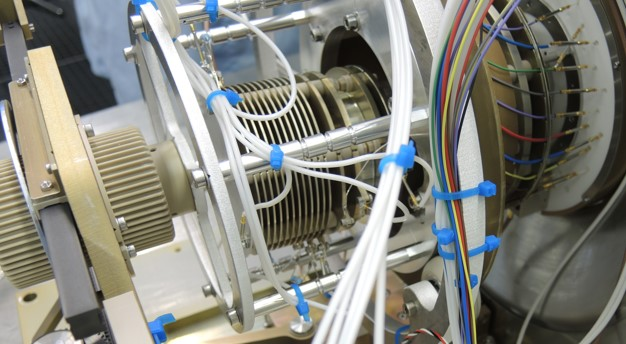
\includegraphics[width = 0.95\textwidth]{Experiments/reflectron_Prototype1.jpg}
		\end{subfigure}
		\begin{subfigure}{0.5\textwidth}
			\centering
			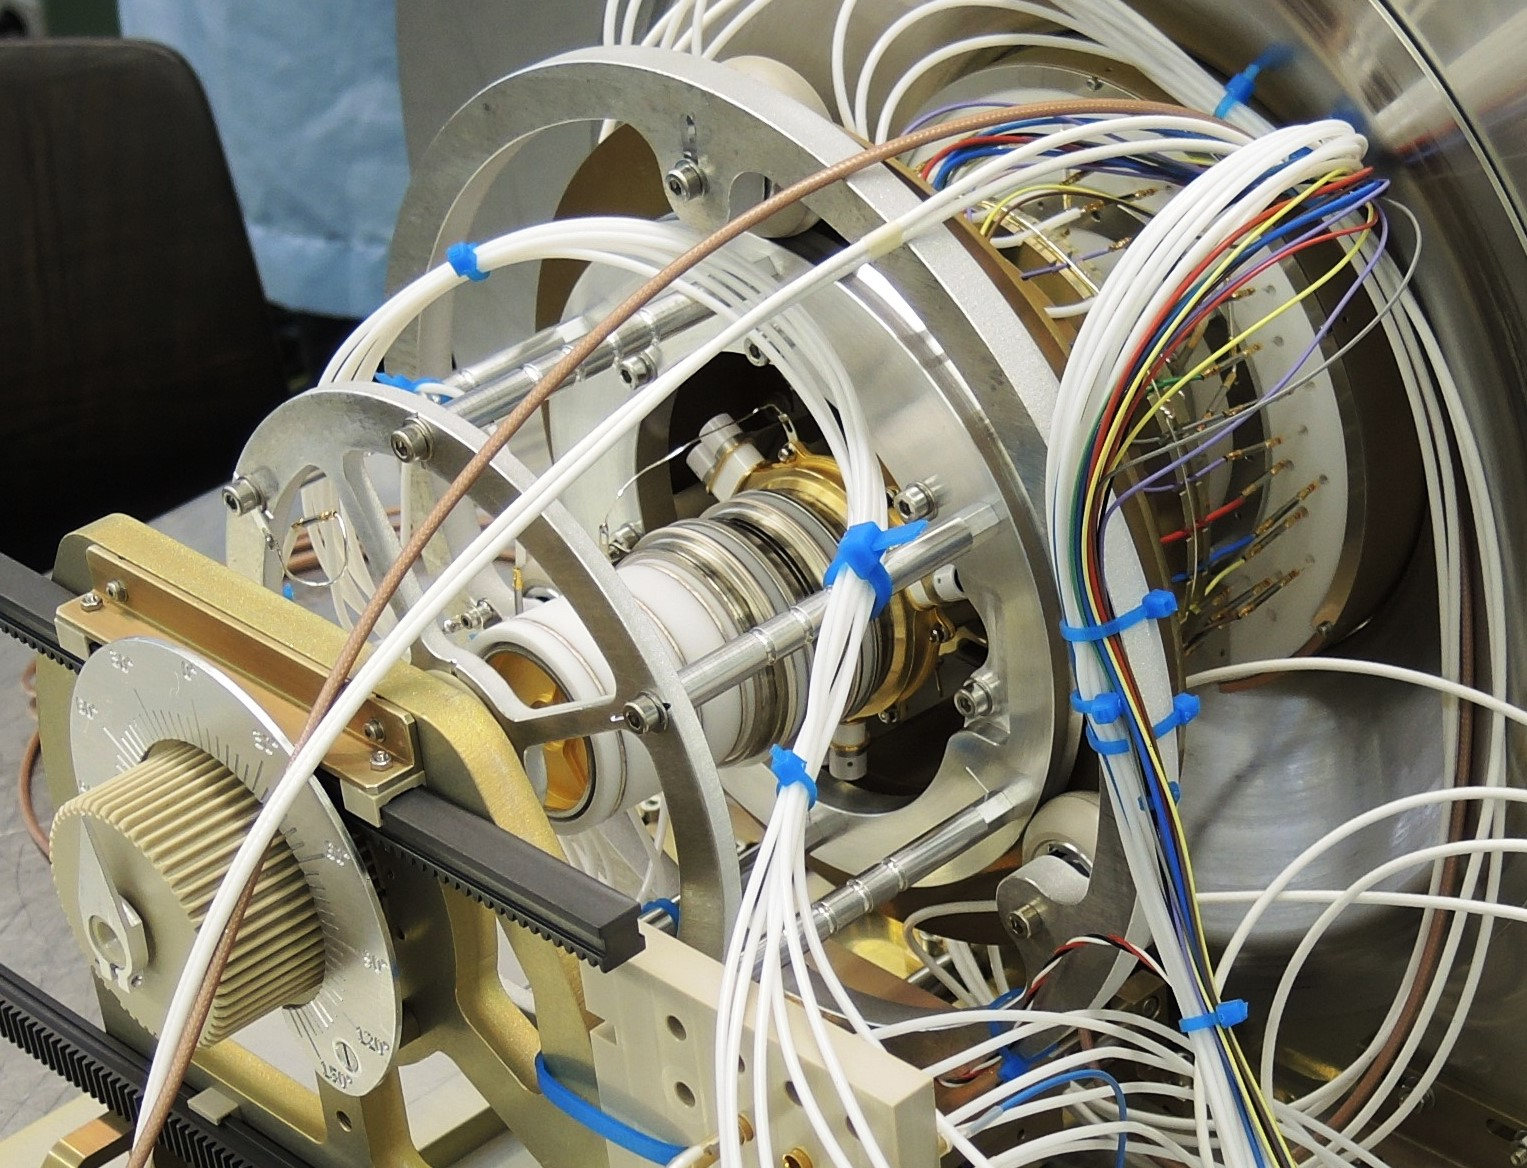
\includegraphics[width = 0.85\textwidth]{Experiments/reflectron_flight.JPG}
		\end{subfigure}
		\caption{Left: Prototype ion-mirror with ring-electrodes. Right: Prototype with flight ion-mirror.}
		\label{fig:ExpRefl}
	\end{figure}
	The measurements were performed in a vacuum chamber. The residual gas pressure for the measurements with the prototype ion-mirror was 5$\cdot$10\textsuperscript{-10}mbar and for the measurements with the flight ion-mirror 1.4$\cdot$10\textsuperscript{-9}mbar. The test gases were injected directly through a leak valve to increase the chamber pressure up to 1$\cdot$10\textsuperscript{-8}mbar. The used test gases were: Ne, Ar, Kr and Xe. 3\, Mio. single spectra were histogramed for each of the measurements. All voltages of the instrument were optimized for the measurements with the two ion-mirrors. Table\ref{tab:refPerftab} shows the signal-to-noise ratios and the mass resolution of the different test gases measured with the two instrument configurations.\\
	\begin{table}
		\begin{center}
		\begin{tabular}{|l|r|r|r|r|}
			\hline
			Gas						&SNR ProtoR	&SNR PFMR	&m/$\Delta$m ProtoR	&m/$\Delta$m PFMR\\
			\hline
			\textsuperscript{20}Ne	&2022.9		&562.4		&200 ± 12		&236 ± 16\\
			\textsuperscript{40}Ar	&4732.6		&1808.4		&212 ±  9		&267 ± 15\\
			\textsuperscript{86}Kr	&746.1		&414.3		&224 ±  7		&292 ± 12\\
			\textsuperscript{136}Xe	&185.5		&97.1		&265 ±  8		&332 ± 13\\
			\hline
		\end{tabular}
		\end{center}
		\caption{Table listing the signal-to-noise ratios (SNR) and the mass resolution (m/$\Delta$m) of the prototype ion-mirror (ProtoR) and the flight ion-mirror (PFMR).}
		\label{tab:refPerftab}
	\end{table}
	The SNR of the measurements with the flight ion-mirror is for all gases lower than the SNR of the measurements with the prototype ion-mirror. This is due to the higher amount of residual in the chamber during the measurements with the flight ion-mirror. The mass resolution of all of the test gases is higher when measuring with the flight ion-mirror.

	
%----------------------------------------------------------------------------------
	\subsection{Flight Antechamber \notes{finished}}
	% dimensions old antechamber: d_in = 4 mm, d_out = 3 mm, d_sp = 40 mm
	%			new:			d_in = 5 mm, d_out = 4 mm, d_sp = 80 mm
	% For further explanation of the geometry see Chap.\ref{subsubsec:Densenhan}.
	After successfully testing the flight ion-mirror, the flight antechamber was tested. A picture of the prototype and the flight antechamber is shown in Fig.\,\ref{fig:expAntchamPic}. The antechambers consist of two parts. In the old design the two parts of the antechamber had a rim on which the screws were mounted to put the two parts together. These screws were at position $\pm$45\degree. Tests with this antechamber revealed that neutral particles hit these screws and scatter into chamber (Fig.\ref{fig:AnteMeasData}a) \cite{Meyer_2017_ante}). Therefore, an antechamber with a flat outer surface was required. In the new design the screws are recessed into the 1\,\si{\milli\meter} thin surface of the antechamber to get rid of the needed rim in the old design. In addition, the new antechamber is by a factor two bigger than the prototype antechamber with the aim to get more signal. Simulations of the flight trajectory revealed that two holes were required at positions $\pm$60\degree to get optimal signal \cite{SOC_Crema3p2}. The CASYMIR test facility is not able to shoot the neutral particle beam under an angle of 60\degree onto the instrument. To test the new design, an slightly different antechamber was used with the second entrance hole at position $\theta_0 = -90\degree$ instead of -60\degree. With a rotation mechanism, the instrument can be rotated around the x-axes by $\pm$90\degree.\\
	\begin{figure}[h!]
		\begin{subfigure}{.5\textwidth}
			\centering
			\includegraphics[width=\textwidth]{Experiments/ProtoAnte.png}
		\end{subfigure}
		\begin{subfigure}{.5\textwidth}
			\centering
			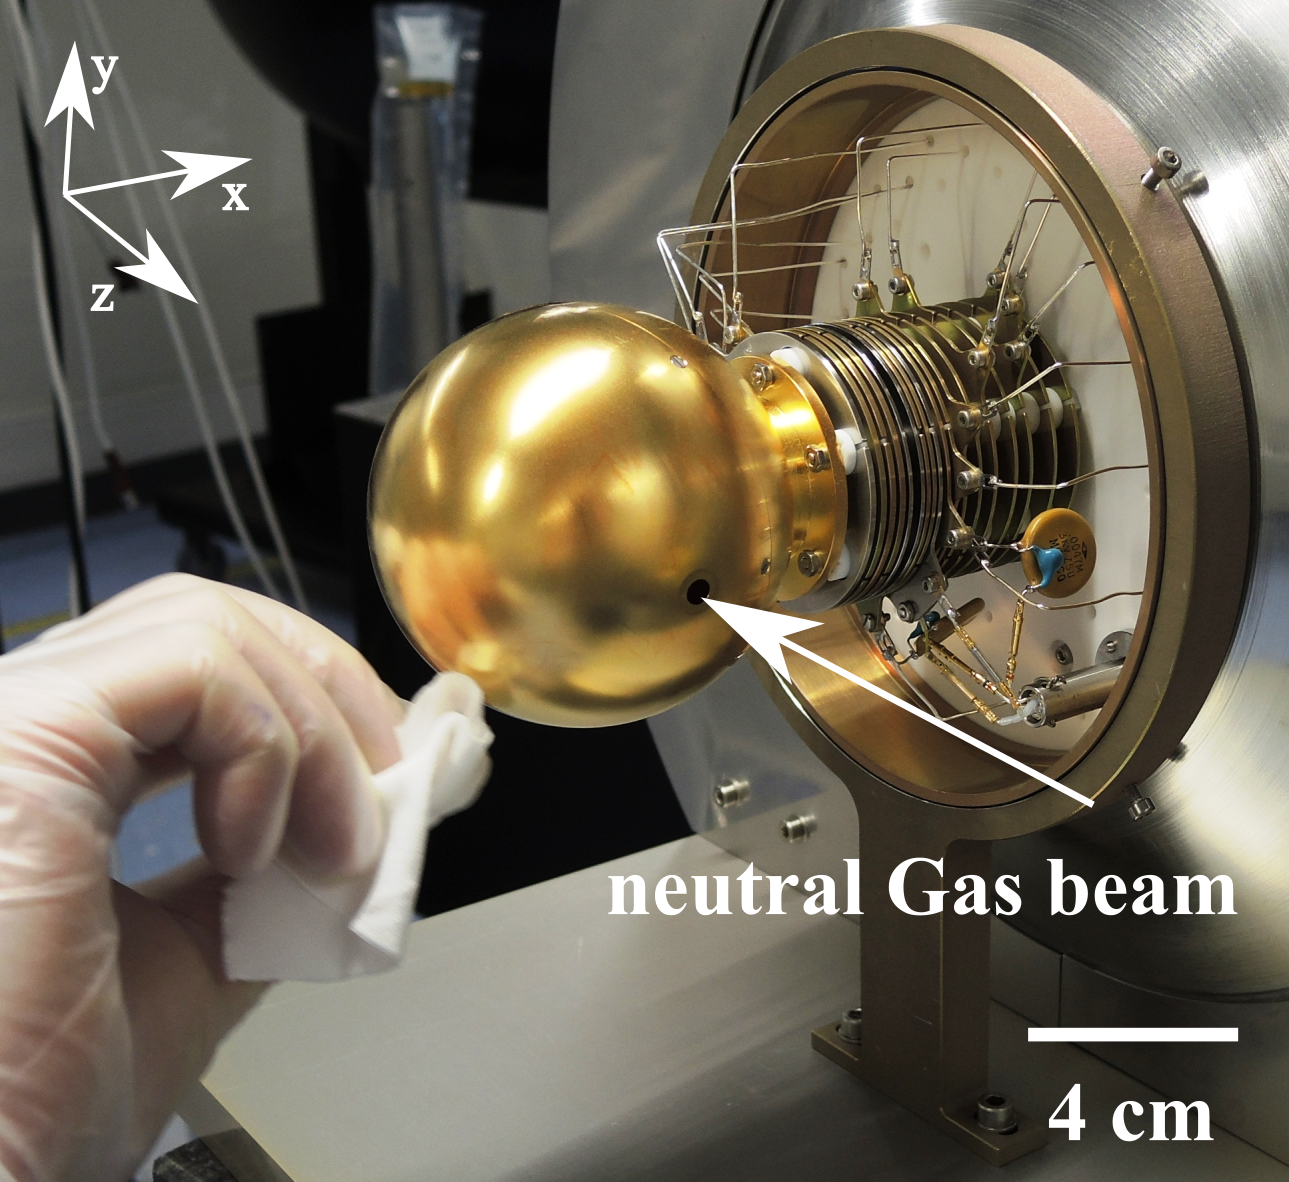
\includegraphics[width=.8\textwidth]{Experiments/FlightAnte.png}
		\end{subfigure}
		\caption{Left: Prototype antechamber. Right: flight-like antechamber with two entrance holes at positions +60\degree and -90\degree.}
		\label{fig:expAntchamPic}
	\end{figure}
	These measurements were conducted at the CASYMIR test facility at the university of Bern. CASYMIR is able to generate a neutral particle beam with velocities up to 5.5\,\si{\kilo\meter\per\second} \cite{CASYMIR_Graf2004}. For these measurements the particle velocity was about 2.5\,\si{\kilo\meter\per\second} because this is the velocity of the spacecraft in Ganymede orbit, which will be 90\% of the measuring time of NIM.\\
	\begin{figure}[h!]
		\begin{subfigure}[t]{.5\textwidth}
			\centering
			\includegraphics[width=\textwidth]{Experiments/oldAnte_ThMode.png}
			\caption{Old antechamber, thermal mode.}
		\end{subfigure}
		\begin{subfigure}[t]{.5\textwidth}
			\centering
			\includegraphics[width=\textwidth]{Experiments/oldAnte_NMode.png}
			\caption{Old antechamber, neutral mode.}
		\end{subfigure}
		\begin{subfigure}[b]{.5\textwidth}
			\centering
			\includegraphics[width=\textwidth]{Experiments/newAnte_ThMode.png}
			\caption{New antechamber, thermal mode.}
		\end{subfigure}
		\begin{subfigure}[b]{.5\textwidth}
			\centering
			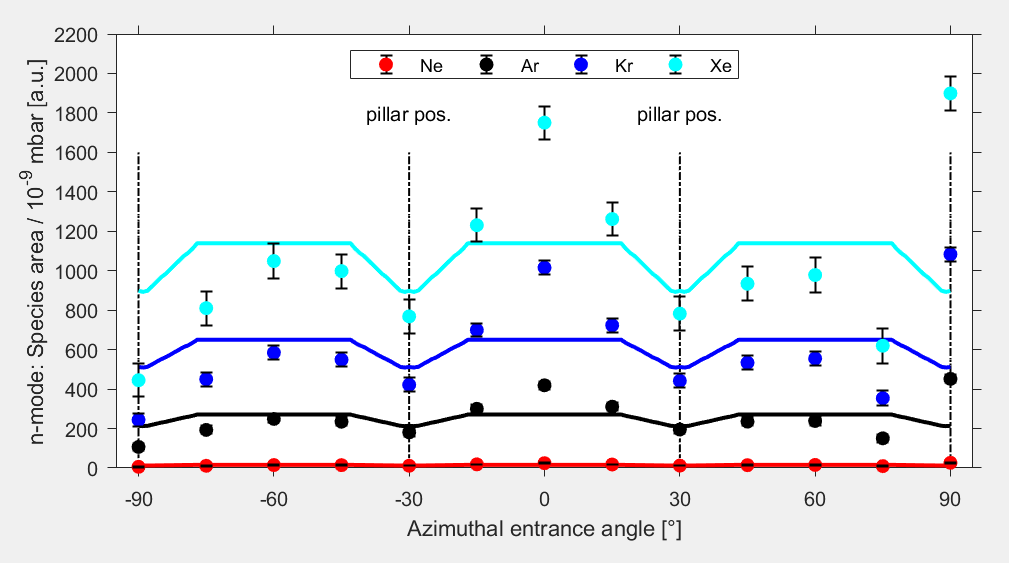
\includegraphics[width=\textwidth]{Experiments/newAnte_NMode.png}
			\caption{New antechamber, neutral mode.}
		\end{subfigure}
		\caption{Panel a) an b) show measurements done with the NIM Prototype sensor with the old antechamber attached. a) shows measurement conducted with the thermal gas mode and panel b) shows measurements of the neutral mode respectively \cite{Meyer_2017_ante}. c) and d) are the corresponding measurements performed with the new antechamber attached to the NIM Prototype.}
		\label{fig:AnteMeasData}
	\end{figure}
	Fig.\,\ref{fig:AnteMeasData}~a) shows measurements conducted with the thermal mode when the old antechamber was attached \cite{Meyer_2017_ante}. For these measurements, the instrument was rotated around the x-axis by keeping the beam at the same position. When rotating the antechamber, the hole moves out of the neutral particle beam because the beam is smaller than the antechamber. The expected intensity distribution $I_{ant}$ is a combination of the function of the moving hole through the beam with a normal distribution:
	\begin{equation}
		I_{ant} = \frac{A}{\sigma\sqrt{2\pi}}\int_{x_{min}}^{x_{max}} \exp^{\frac{(x-\mu)^2}{2\sigma^2}} dx
	\end{equation}
	With $A$ a constant taking the beam intensity into account, $\sigma$ the standard deviation of the beam and $\mu$ the position of the beam centre relative to the centre of the antechamber which is zero. The borders of the integral determine the section of the beam entering the antechamber:
	\begin{align}
		x_{max} &= r_{ant}\sin{\alpha} - r_{aHi}\cos{\alpha}\label{eq:antIntgrLimHigh}\\
		x_{min} &= r_{ant}\sin{\alpha} + r_{aHi}\cos{\alpha}\label{eq:antIntgrLimLow}
	\end{align}
	With $r_{ant}$ the radius of the antechamber and $r_{aHi}$ the radius of the antechamber entrance hole. The sine contribution considers the shift of the hole in y-direction when the hole is rotated. The cosine contribution comes from the projection of the beam on the entrance hole. For the measurements with the new antechamber, the shift in y-direction when rotating the instrument was compensated by shifting the whole instrument. Therefore the sine contribution in Eq.\eqref{eq:antIntgrLimHigh} and Eq.\eqref{eq:antIntgrLimLow} cancels leading to a cosine-like function.\\
	When comparing Fig.\,\ref{fig:AnteMeasData}~a) and c), the artefacts successfully vanished after the redesign. The higher intensity at angle +90\degree is most probable an outlier because it appears in both the thermal (Fig.\,\ref{fig:AnteMeasData}~b)) and the neutral mode figure (Fig.\,\ref{fig:AnteMeasData}~d)) of the measurements with the new antechamber. The lower measured signal intensity for the measurements with the new antechamber is a result of having an additional entrance hole which was necessary because of the flyby trajectories (see Chap.\ref{subsubsec:Densenhan}).\\
	Fig.\ref{fig:AnteMeasData}~b) shows measurements conducted with the neutral gas mode with the old antechamber attached and Fig.\ref{fig:AnteMeasData}~d) shows measurements conducted with the neutral gas mode when the new antechamber was attached. At position $\pm$30\degree and $\pm$90\degree are pillars holding the stack of the ion-optical lenses together. When the beam hits these pillars, the particles scatter in all directions leading to a damping of the signal. For the neutral gas channel, no difference in the signal distribution and intensity is expected because a change in the antechamber design does not influence the signal measured with the neutral gas channel. The observed signal of the neutral gas mode when the new antechamber is attached, is significantly higher than with the old antechamber. This is due to a better voltage set. A different voltage set for the voltages in the ionization region changes the distribution of the electron beam thus leading to a different ion distribution in the ionization region. This leads to a different angular distribution of the signal for the neutral gas channel when comparing the results of the two measurement series. 
	
%-------------------------------------------------------------------------------------	
	\subsection{Signal Distribution \notes{finished}} % Think of a good Chapter name
	\begin{figure}[h!]
		\centering
		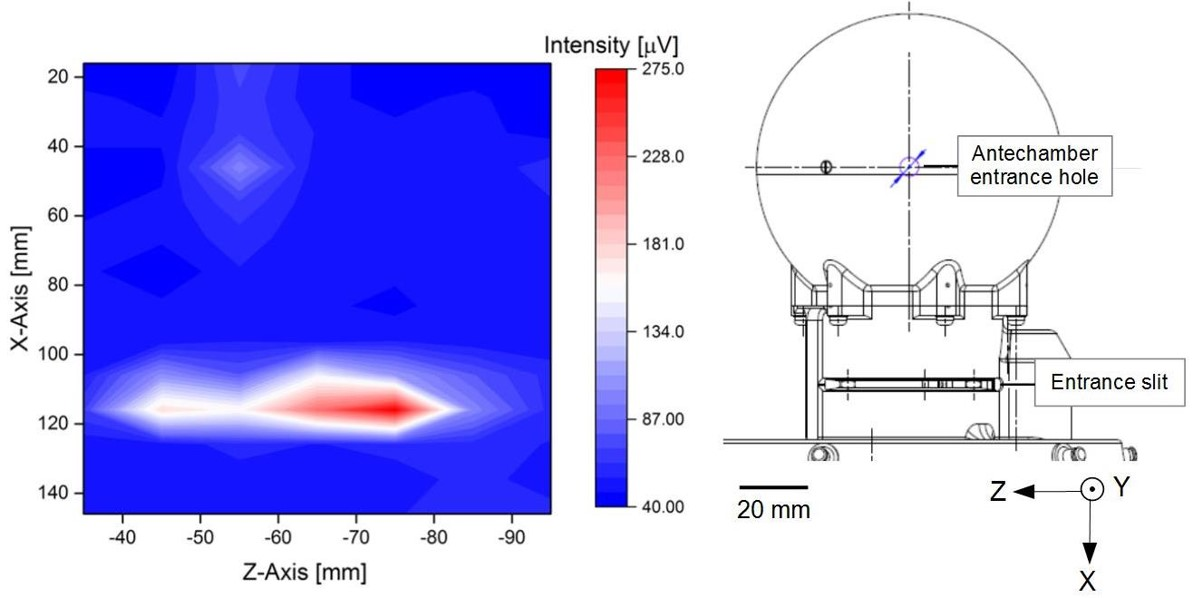
\includegraphics[width=\textwidth]{Experiments/2D_scan_anteEntr.jpg}
		\caption{Left:Intensity profile when shooting with the neutral particle beam at the structure of the NIM PFM instrument. Right: Front view as seen by the neutral particle beam.}
		\label{exp:PFMIntCharTot}
	\end{figure}
	\begin{figure}[h!]
		\centering
		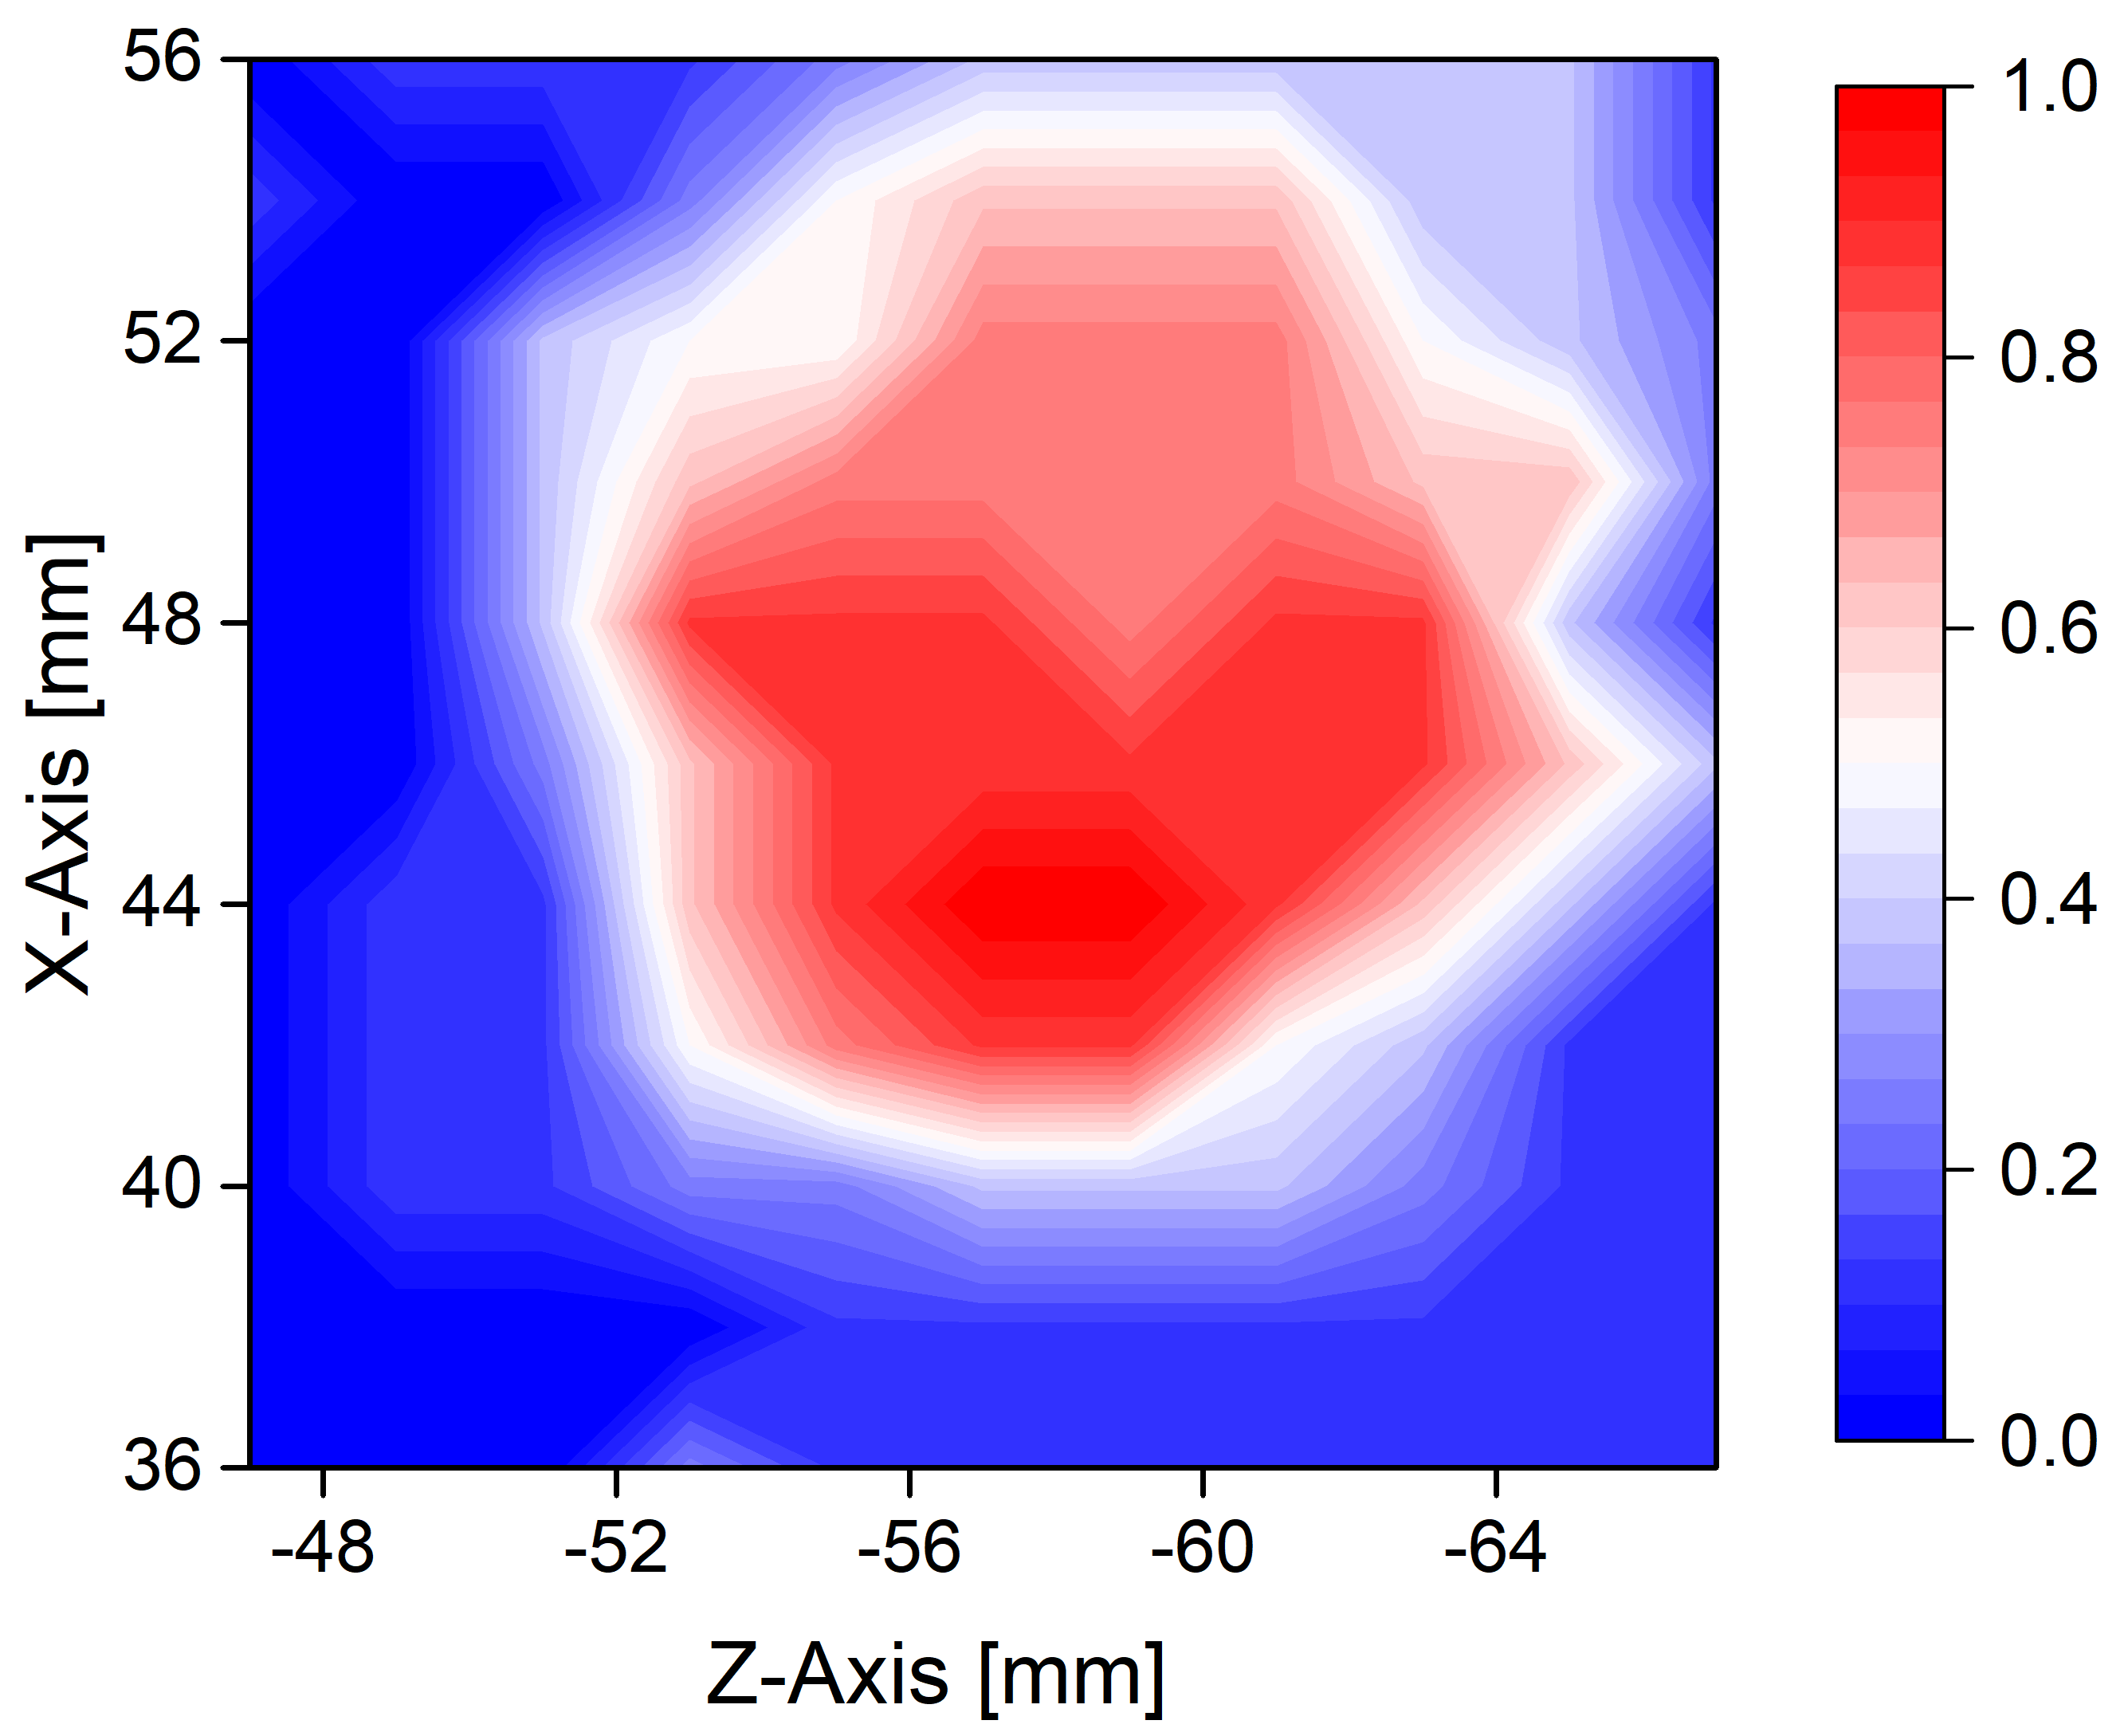
\includegraphics[width=.7\textwidth]{Experiments/2D_scan_Ant.png}
		\caption{Zoom on the antechamber hole when shooting with the neutral particle beam at the structure of the NIM PFM instrument.}
		\label{exp:PFMIntCharAnt}
	\end{figure}	
	\begin{figure}[h!]
		\centering
		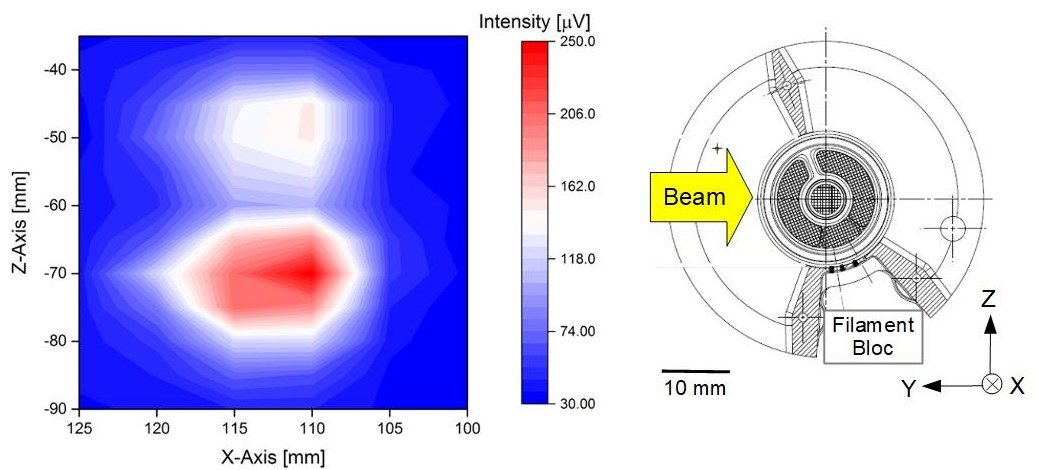
\includegraphics[width=\textwidth]{Experiments/2D_scan_Entr.jpg}
		\caption{Left: Zoom on the entrance when shooting with the neutral particle beam at the structure of the NIM PFM instrument. Right: Top view on the entrance.}
		\label{exp:PFMIntCharEnt}
	\end{figure}
	\notes{Chapter name could be improved}. For the first tests with the NIM PFM, the front side of the NIM instrument was scanned with the neutral particle beam to find the position of the entrance slit and the antechamber entrance hole to align the beam properly with the instrument. Fig.\,\ref{exp:PFMIntCharTot}~left shows the scan of the front side and Fig.\,\ref{exp:PFMIntCharTot}~right shows the corresponding structural part. The antechamber entrance hole is clearly visible as a small dot. Fig.\,\ref{exp:PFMIntCharAnt} shows a zoom with a better resolution of the entrance hole which shows a nice Gaussian distribution. When looking at the entrance slit, there are two positions with increased intensities. The zoom on Fig.\,\ref{exp:PFMIntCharEnt} reveals that the positions of biggest intensity is were the beam hits the structure covering the two electron emitting filaments. The other intensity maximum is where the beam hits the supporting structure opposite of the filament bloc. When the gas hits these structures, the gas slows down leading to a local increase of the gas density. Therefore, the structure partially thermalizes the gas similar as the closed source antechamber. This was not intended because with the neutral gas channel the aim is to measure incoming particles directly without any interaction with the structure. In the design of the PFM, the filament bloc and the supporting structure act like a funnel directing the sputtered gas to the central grid. The intensity amplification when shooting on the filament bloc is unavoidable. For the supporting structure opposite of the filament, a pillar instead of the plate like structure would have been the better option. When the gas hits the pillar, the pillar scatters the gas in all direction instead of scattering only in the direction of the central grid. This phenomenon was observed when doing a similar measurement with the NIM prototype (Fig.\,\ref{exp:ProtoIntCharEnt}).\\
	The ion-source of the prototype had six pillars holding the different focusing lenses together. In Fig.\,\ref{exp:ProtoIntCharEnt} the pillars are marked as red circles. The electron emitting filament was opposite of the main gas inflow direction. For these measurements, the ionization region was scanned with the neutral particle beam at angles 0\degree and $\pm$60\degree to shoot between the pillars. When scanning from the front side, the signal intensity has a nice Gaussian shape. When shooting at angles of $\pm$60\degree the Gaussian distribution is visible when the neutral particle beam is aligned over the centre grid with an asymmetry toward the side of the filament. The filament bloc slows down the neutral particles leading to a small amplification of the signal. This amplification is less dominant than in the design of the PFM because the part of the filament structure seen by the beam is tilted outward. At distances bigger than $\pm$25\,mm from the centre, the signal drops again. This is where the beam is completely outside of the ionization region.
	\begin{figure}[h!]
		\centering
		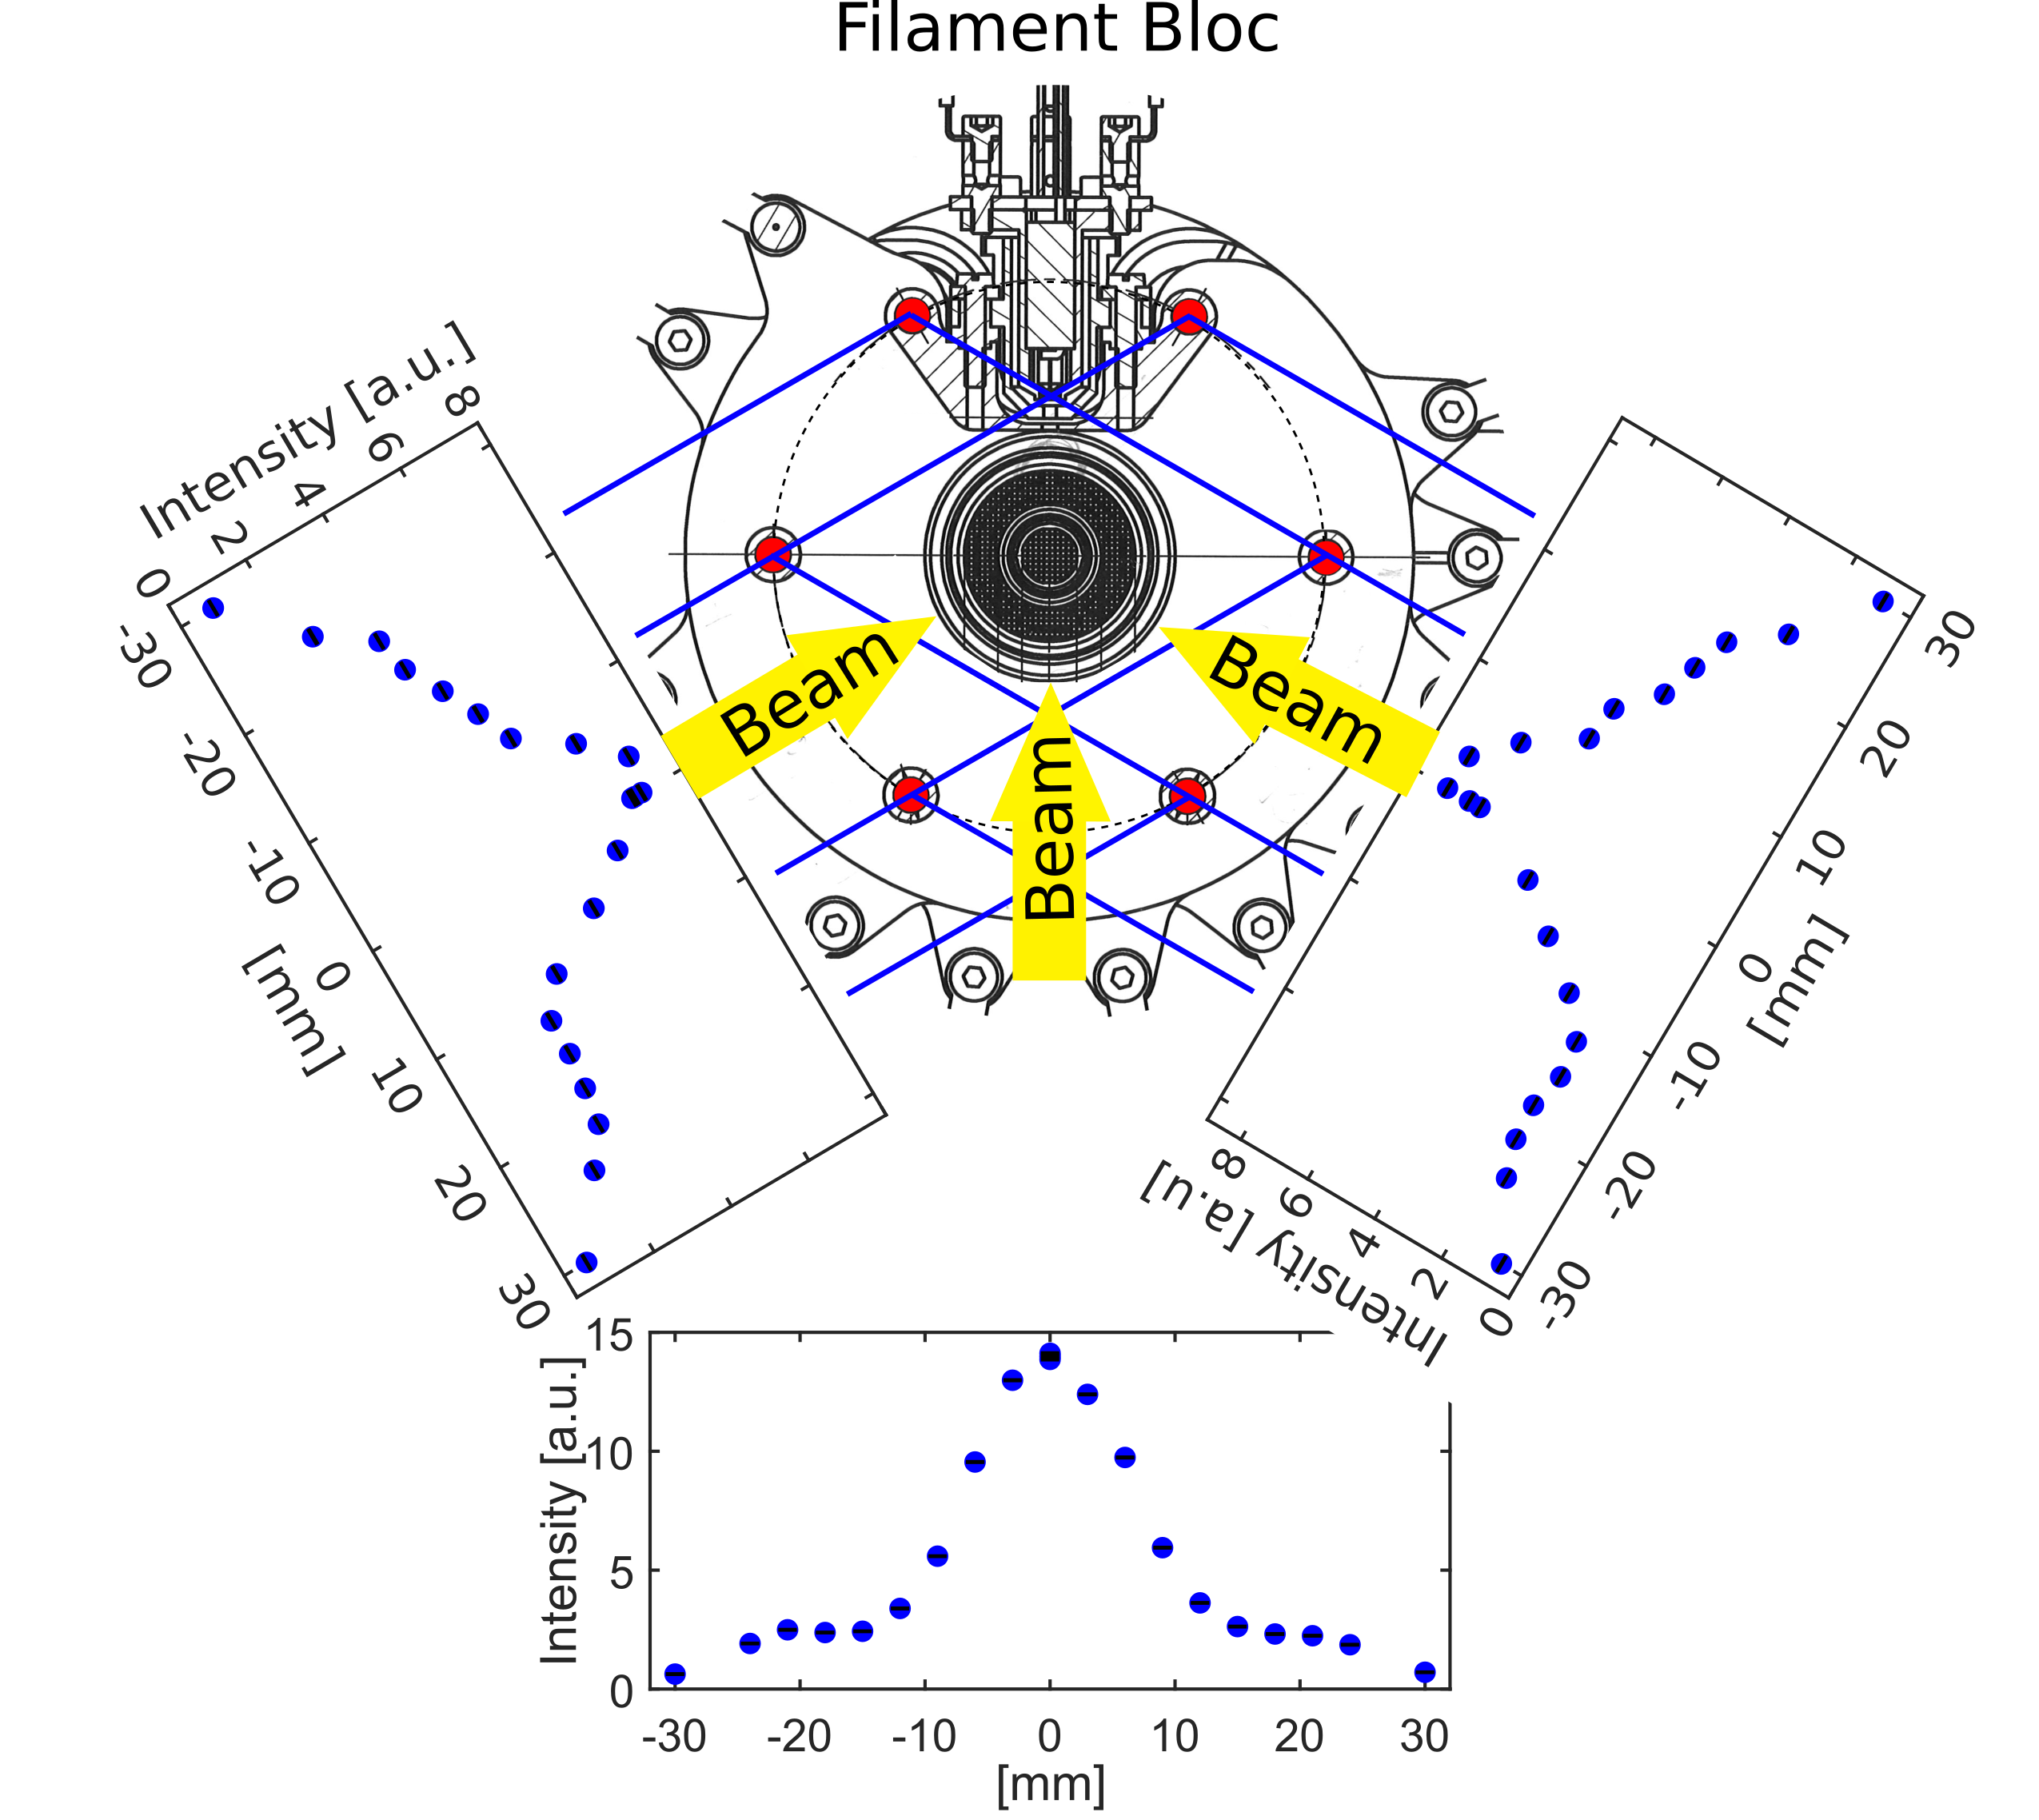
\includegraphics[width=\textwidth]{Experiments/Entrence_Proto_topview.png}
		\caption{Zoom on the entrance when shooting with the neutral particle beam at the structure of the NIM Prototype. The red circles mark the positions of the pillars holding the ion source together.}
		\label{exp:ProtoIntCharEnt}
	\end{figure}
	
%--------------------------------------------------------------------------------------------	
	\subsection{Shutter Performance Test \notes{finished}}
	When measuring with the neutral gas channel, the aim is that the particles are measured directly without any interaction with the structure of the instrument. Therefore, a shutter between the antechamber and the ionization region was required to close the particle entrance from the antechamber. In this section the performance of the shutter was tested. According to the model stated in Chap.\ref{subsubsec:motorflow} the shutter should damp the signal by a factor 600.\\
	These tests were performed with the NIM PFM. The PFM was operated with laboratory electronics. The tests were performed at the CASYMIR test facility. The used particle beam consisted of hydrogen and xenon with a velocity of 2\,\si{\kilo\meter\per\second}. Three different measurements were performed: One with the beam directing onto the antechamber with the shutter open, one with the shutter closed and a background measurement, where the particle beam was pointed onto the outer structure of NIM to estimate how much of the signal arises from the test gas scattering into the ionization region when the beam is directed in an arbitrary direction. This background was subtracted from both signals before they were divided through each other to determine the damping factor $G_{close}$ of the shutter.\\
	The resulting damping factor of the shutter is 12 instead of the required 1000. The biggest impact has the actual thickness of the gap between the shutter and the antechamber when the shutter is closed. The damping reduces significantly when the gap is bigger than actually designed. This is shown in Fig.\,\ref{fig:ShutGapSizeSigDamp} in Chap.\,\ref{subsubsec:motorflow}. With a gap size of about 0.1\,mm instead of 0.01\,mm the damping factor is only about a factor 25. Other reasons are that the portion of the beam which scatters on the antechamber outer walls gets thermalized in the vacuum chamber and adds to the signal intensity. In the outer space, the gas scatters on the antechamber but does not reach the ionization region because it will flow around the instrument.
	
	\begin{comment}	
	\begin{table}
		\begin{center}
			\begin{tabular}{|c|c|c|}
				\hline
				\multirow{2}{*}{Configuration} & \multicolumn{2}{c|}{Species Area [a.u.]} \\
				\cline{2-3}
				& \textsuperscript{129}Xe & \textsuperscript{132}Xe \\ \hline
				Shutter open  & 36.97 ±0.07 & 36.7 ±0.06\\
				Shutter close &	6.76 ±0.07 & 6.7 ±0.05\\
				Background & 3.87 ±0.05 & 3.73 ±0.03 \\
				\hline
			\end{tabular}
		\end{center}
		\caption{The signal intensity is given for different shutter positions. It is proportional to the number of measured particles. The background was determined by shooting with the beam onto the outer structure of NIM.}
%		\label{tab:measShutMot}
	\end{table}
		% IsoArea [10^9]
		
	\begin{table}
		\begin{center}
			\begin{tabular}{|c|c|c|c|c|}
				\hline
				\multirow{2}{*}{Configuration} & \multicolumn{4}{c|}{Species Area [a.u.]} \\
				\cline{2-5}
				&N\textsubscript{2}& CO\textsubscript{2} & \textsuperscript{129}Xe & \textsuperscript{132}Xe \\ \hline
				Shutter open & 18.36 ±0.07 & 10.76 ±0.06 & 36.97 ±0.07 & 36.7 ±0.06\\
				Shutter close & 19.57 ±0.07 & 12.04 ±0.06 &	6.76 ±0.07 & 6.7 ±0.05\\
				Background & 18.43 ±0.07 & 11 ±0.06 & 3.87 ±0.05 & 3.73 ±0.03 \\
				\hline
			\end{tabular}
		\end{center}
		\caption{The signal intensity is given for different shutter positions. It is proportional to the number of measured particles. The background was determined by shooting with the beam onto the outer structure of NIM. N\textsubscript{2} and CO\textsubscript{2} are part of the residual gas and Xe is the test gas in the neutral particle beam.}
%		\label{tab:measShutMot}
	\end{table}
	
	\begin{table}
	\begin{center}
		\begin{tabular}{|c|c|c|c|c|c|c|c|c|}
			\hline
			\multirow{2}{*}{Configuration} & \multicolumn{4}{c|}{m/$\Delta$m}& \multicolumn{4}{c|}{SNR} \\
			\cline{2-9}
			&N\textsubscript{2}& CO\textsubscript{2} & \textsuperscript{129}Xe & \textsuperscript{132}Xe & N\textsubscript{2} & CO\textsubscript{2} &\textsuperscript{129}Xe&\textsuperscript{132}Xe\\ \hline
			Shutter open & 307$\pm$25& 330$\pm$23 & 361$\pm$16& 373$\pm$17 & 550.8 & 309.9 & 735.7 & 740.2\\
			Shutter close &307$\pm$25& 330$\pm$23 & 361$\pm$16& 365$\pm$16 & 540.3 & 315.4 & 120.8 & 121.6\\
			Background &307$\pm$25& 330$\pm$23 & 353$\pm$15& 357$\pm$16 & 631.6 & 360.2 & 85.4 & 84\\
			\hline
		\end{tabular}
	\end{center}
	\caption{Mass resolution m/$\Delta$m and Signal-to-Noise Ratio for different shutter positions. N\textsubscript{2} and CO\textsubscript{2} are part of the residual gas and Xe is the test gas in the neutral particle beam.}
%	\label{tab:measShutMot}
	\end{table}
	
	\end{comment}	
	

	
%--------------------------------------------------------------------------------
	\subsection{Entrance adaption}
	Due to a redesign of the ion source, an adaption of the entrance electrode IS~3 was necessary (Electrode with 0~V in Fig.\ref{fig:IsAdapt}). Simulations were done to see how big the impact of that design adaption was. Fig.~\ref{fig:IsAdapt} shows the old design (bottom) and the new design (top) of the ionisation region with the voltages applied. In dark blue is the flight path if the electrons and light blue shows the potential lines. The adaption of the corresponding electrode had not big impact on the flight path of the electrons.
	
	\begin{figure}[h]
		\centering
		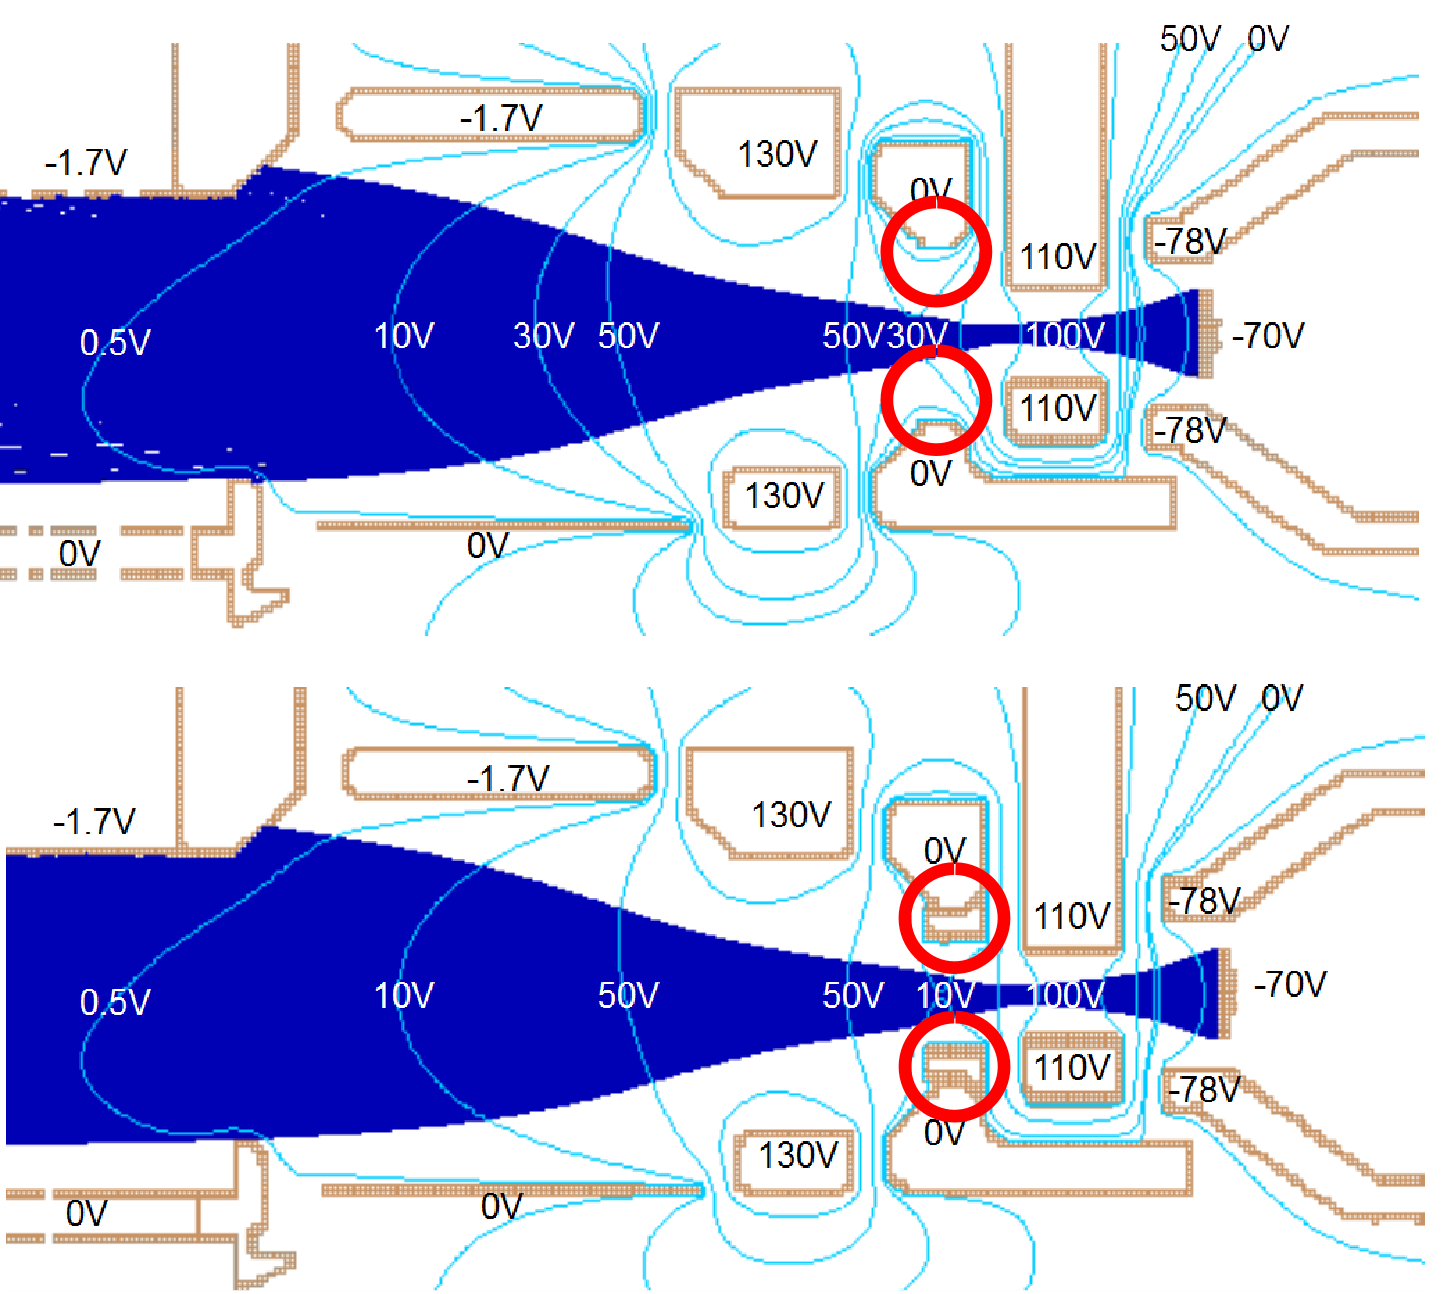
\includegraphics[width=.7\textwidth]{Experiments/IS_adaption.png}
		\caption{text}
		\label{fig:IsAdapt}
	\end{figure}
	
	% Filament repeller simulation tests. Noch Graphiken einmal einfügen. Die wichtigsten.
	% Um herauszufinden, wie wichtig die Position des Filaments ist.
	
	% Noch besser umschreiben. Die position des filaments entspricht nicht der erwarteten??? Was ist da schief gelaufen??? :(
	
	% Intensitätssimulation Countberechnung:
	% Man generiert 2000 e- auf dem Filament und zeichnet immer nach 1E-5 microsec auf, an welcher Position sich die Teilchen gerade befinden. Die Fkt. 'Plot_optVoltAndPos.m' zählt alle Positionen zusammen, welche sich in dem Zylindervolumen befinden. Die Grundfläche des Zylinders ist das Eintritts-Grid von der antechamber und die Höhe ist die Höhe der Entrance. Im th-Mode befinden sich nur in diesem Volumen neutrale Teilchen.
	
	\begin{comment}
	Graphics where the filament position was varied 
	Only put in these graphics if there is enough time to also make the simulations with the electric fields.
	
		\begin{figure}[h]
			\begin{subfigure}{0.53\textwidth}
				\centering
				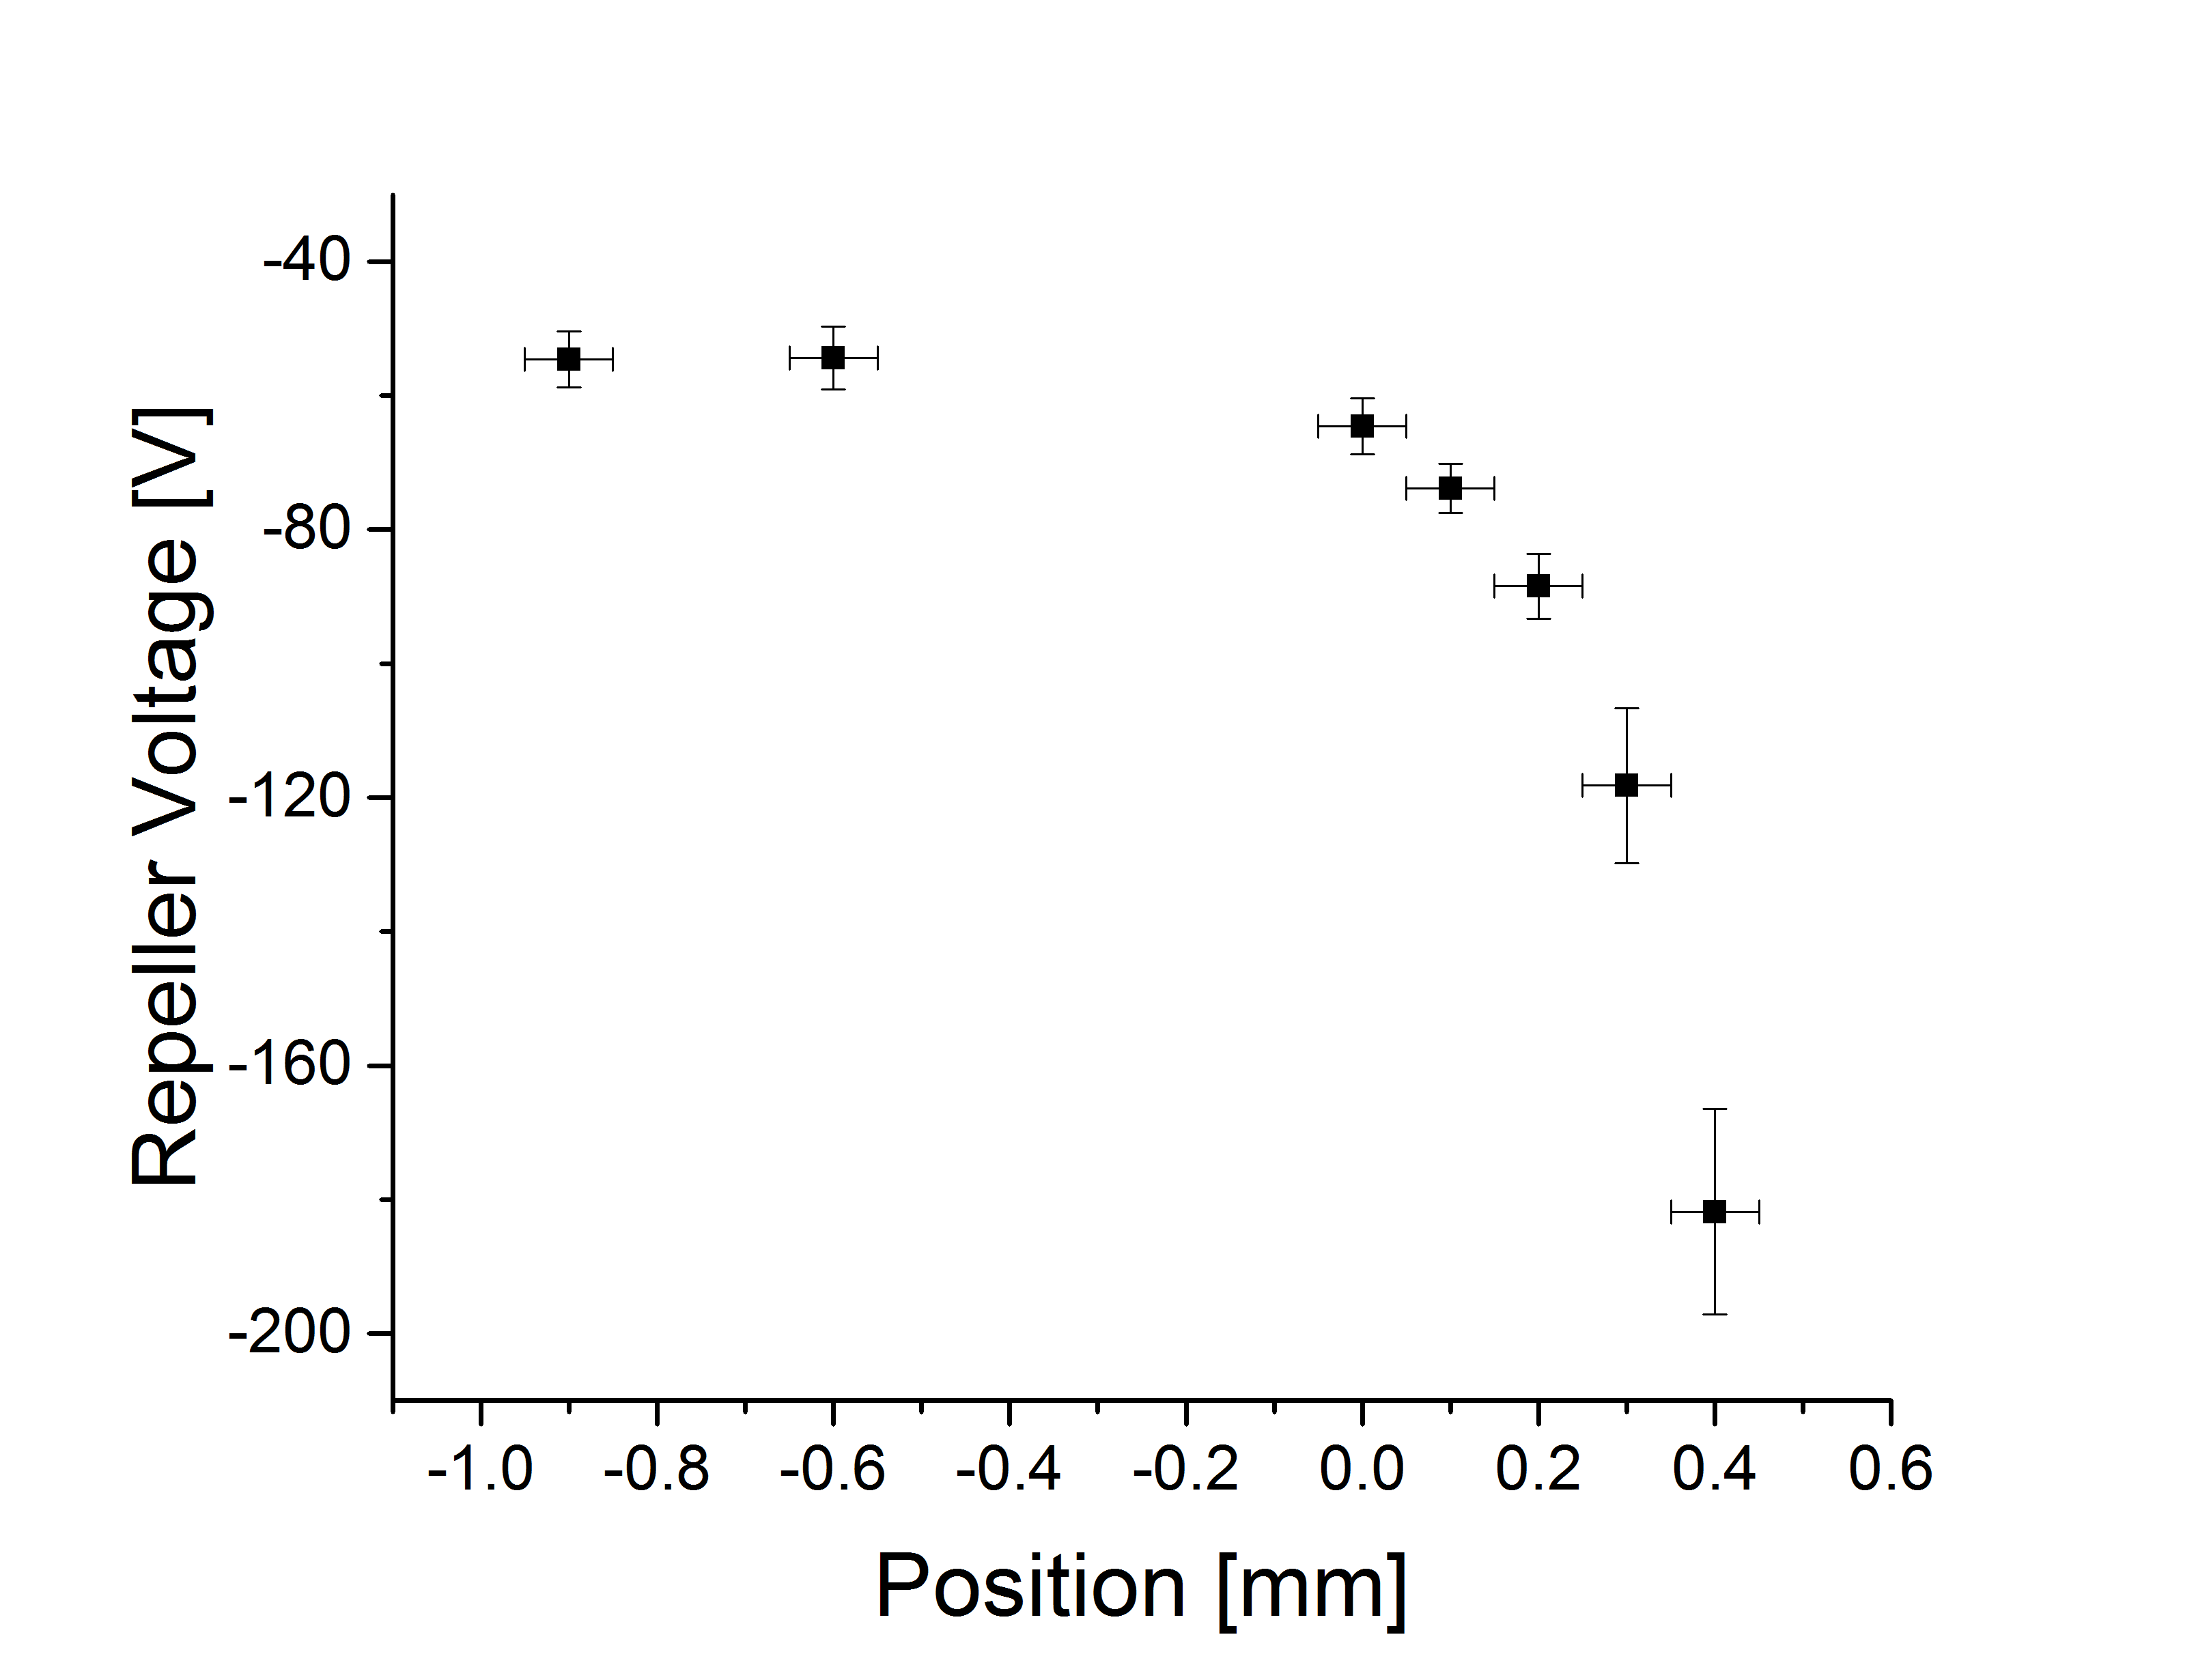
\includegraphics[width= 0.95\textwidth]{Experiments/SimRepPosU.png}
			\end{subfigure}
			\begin{subfigure}{0.47\textwidth}
				\centering
				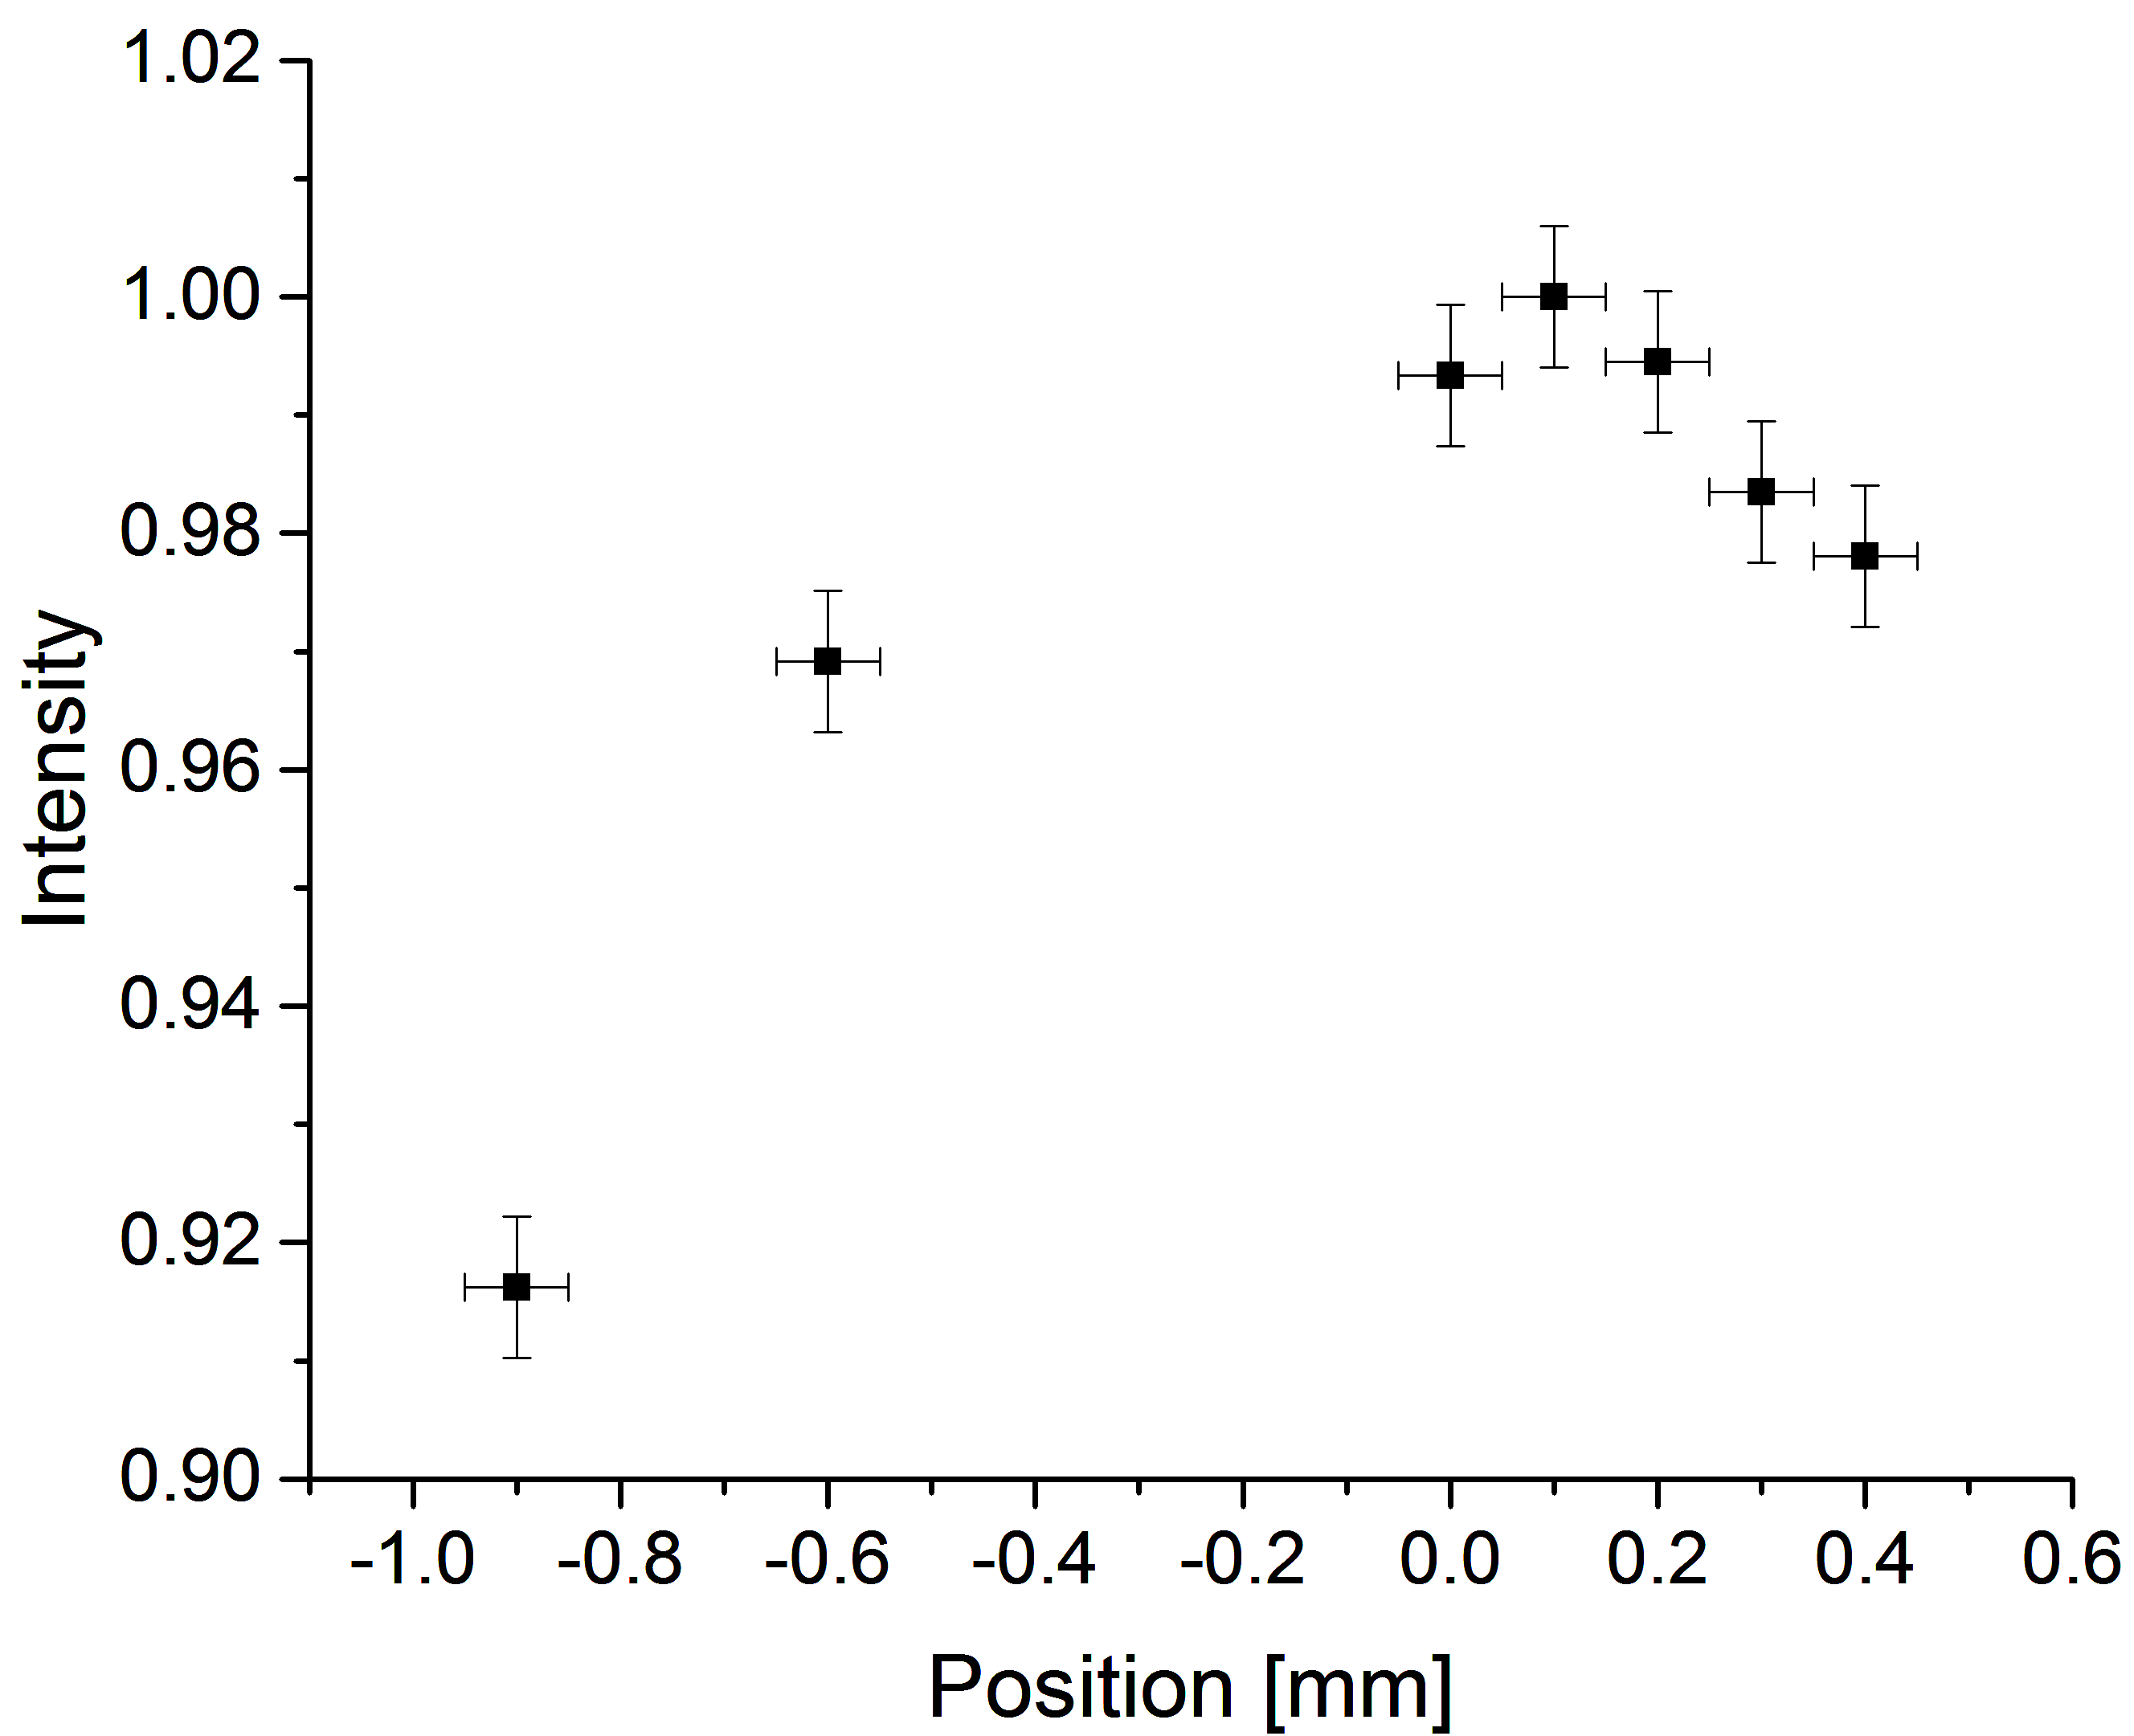
\includegraphics[width= 0.95\textwidth]{Experiments/SimRepPosImax.png}
			\end{subfigure} %0.95
			\caption{Left: The filament repeller voltage to reach the maximum electron intensity over the volume of the neutral particles. Right: Electron intensity normed on the intensity at position 0.} % Noch Graphik wie Intensität bei den versch. Pos abfällt.
			\label{fig:ExpSimRep}
		\end{figure}
	\end{comment}

%--------------------------------------------------------------------------------------------
		\subsection{Pulser \notes{finished}}
		% slit thickness of 2mm and m = 1u -> 3ns to leave the source
		%							m = 2u -> 4.5ns H2
		%							m = 10u -> 10ns
		%							m = 100u -> 32ns
		%							m = 130u -> 37ns
	\begin{figure}[h!]
		\centering
		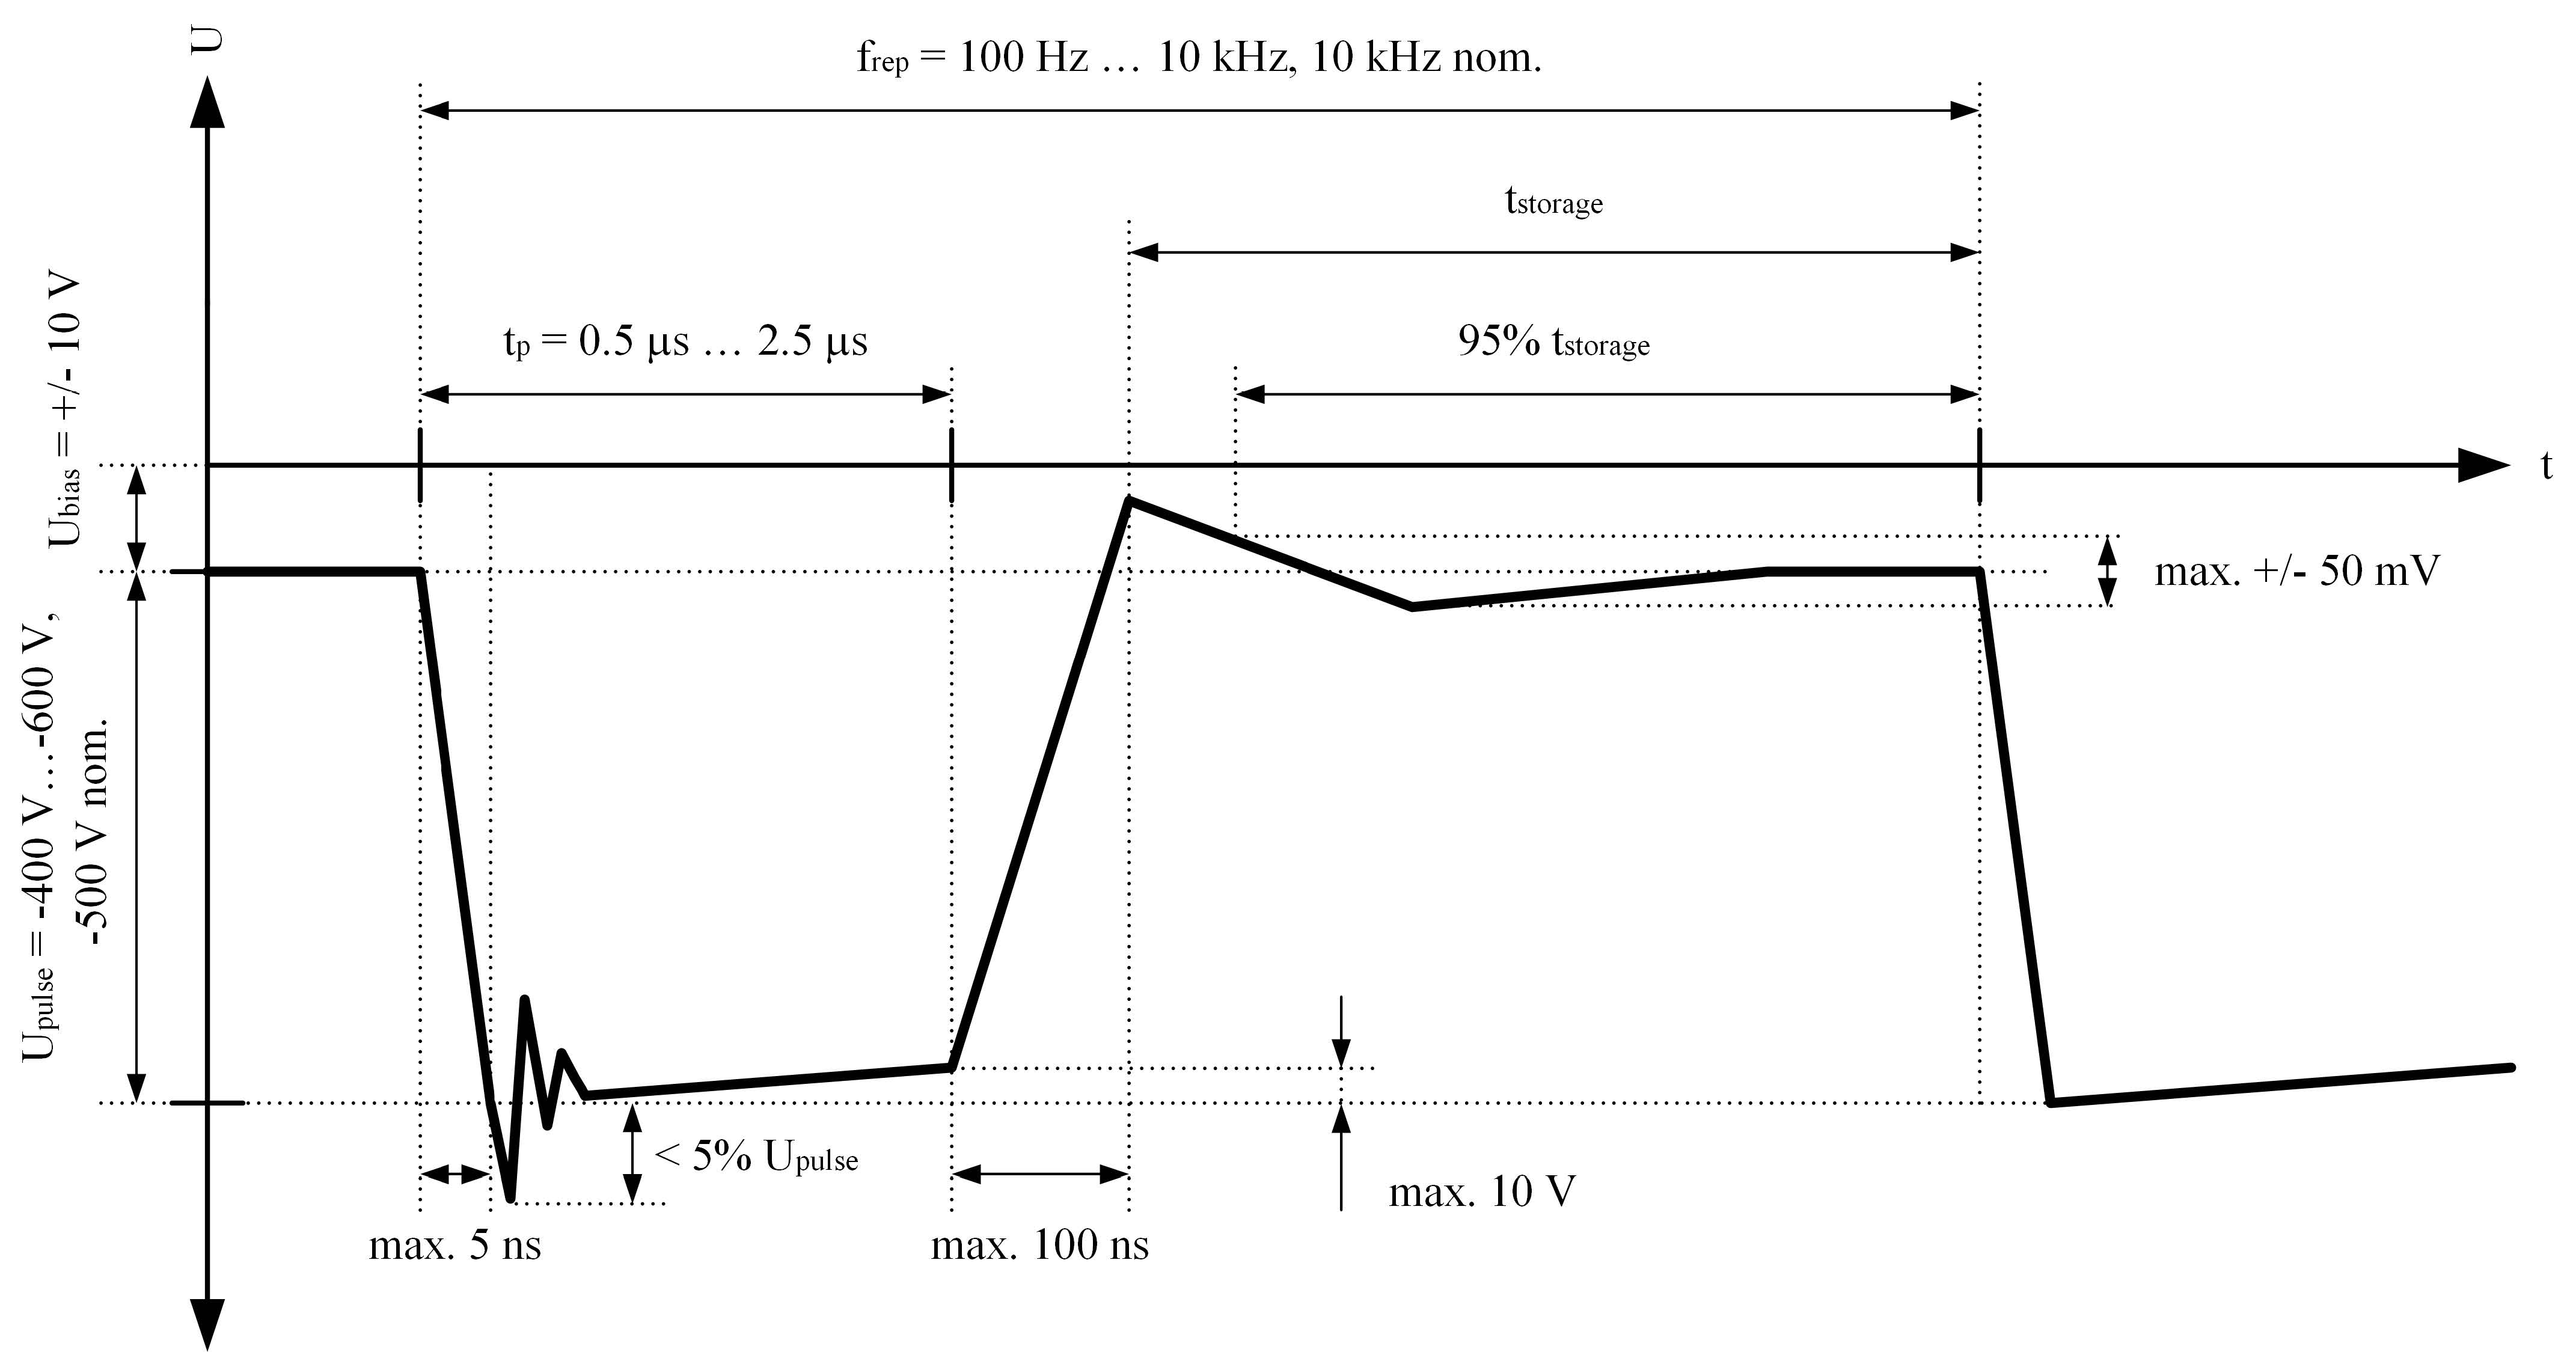
\includegraphics[width=\textwidth]{Bilder/Pulser_theretical_shape.jpg}
		\caption{Specifications for the pulse shape generated by a realistic pulser \cite{Diss_Meyer}.}
		\label{fig:PulserTheoCurve}
	\end{figure}
	The high-voltage pulser is used to accelerate the generated ions in the ionisation region to a certain energy. During the time when no high voltage pulse is applied, the potential has to be stable at the bias voltage to allow ion storage as previously discussed in Chapter\,\ref{chap:IonStor}.\\
	Fig.\,\ref{fig:PulserTheoCurve} shows a schema of a realistic high voltage pulse and Table\,\ref{tab:FlightPulserPerf} shows the characteristics of the flight pulser compared to the requirements. The fall time is the time to build up the negative high voltage on the extraction grid. this time has to be very short to give all ions the same amount of energy. When the fall time is long, low mass particles receive less energy resulting in a lower mass resolution for these species. A fall time of 1~ns lead to a 0.1\,\% lower mass resolution of hydrogen compared to a particle with mass 200~u. A fall time of 5~ns results in a deviation of 3\,\% (cf. Chap.\,\ref{chap:massRes}). The fall time of the flight pulser is a bit longer than according to the specifications. When applying a high voltage, the pulse overshoots its set value and drops slightly. The overshoot and the voltage drop result in a variation of the particle energy for the different species. The ringing of the high voltage, and the pulse drop of the flight pulser are within the specifications. The pulse duration has to be longer than 0.2\,\si{\micro\second} because that is the minimum time particles with masses of 1000\,u need to leave the ionisation region. With some margin, the specifications were set to 0.5\,\si{\micro\second}. The rise time to bias voltage should be smaller than 100\,ns to leave enough time for ion storage. This is well achieved with the flight pulser. The ripple of the bias voltage should be smaller than $\pm$50\,mV to generate a stable electric field during the time when no high-voltage is applied on the extraction grid. A variation by $\pm$100\,mV of the voltage of the electrode opposite of the pulser grid results in a visible variation of the signal intensity during hand optimisation with laboratory electronics. However, the baseline ripple of the flight pulser exceeds this value.\\
	\begin{table}[h!]
		\begin{center}
			\begin{tabular}{|m{2.2cm}|>{\centering}m{2cm}|>{\centering}m{2cm}|>{\centering}m{2.8cm}|>{\centering}m{1.7cm}|m{1.8cm}<{\centering}|}
				\hline
				& Ringing of HV Pulse & Pulse drop at full HV & Baseline Ripple & Fall Time & Rise Time \\ \hline
				Requirement		& $<$ 5\%  & $<$ 10\,V & $\pm$50\,mV & $<$ 5\,ns & $<$ 100\,ns\\
				Flight Pulser	& 2.5\% & 1.9\,V & 300\,mV & 5.76\,ns & 19.7\,ns\\
				\hline
			\end{tabular}
		\end{center}
		\caption{Characteristics of the flight pulser compared with the requirements.}
		\label{tab:FlightPulserPerf}
	\end{table}

%--------------------------------------------------------------------------------------------
	\subsection{Detector Tests \notes{Draft}}\label{chapExp:Det}
	
	\begin{figure}[h] % Flat and folded detector. Make notes of the different parts.
		\centering
		\includegraphics[width=.8\textwidth]{Experiments/Detectors_fla_folded.png}
		\caption{NIM PFM detectors ready for tests. Top: in flat configuration. Bottom: in folded configuration.}
		\label{fig:DetFlatFolded}
	\end{figure}
	\begin{figure}[h] % Detector gain curves during conditioning of both FS detectors.
	\begin{subfigure}{.5\textwidth}
		\centering
		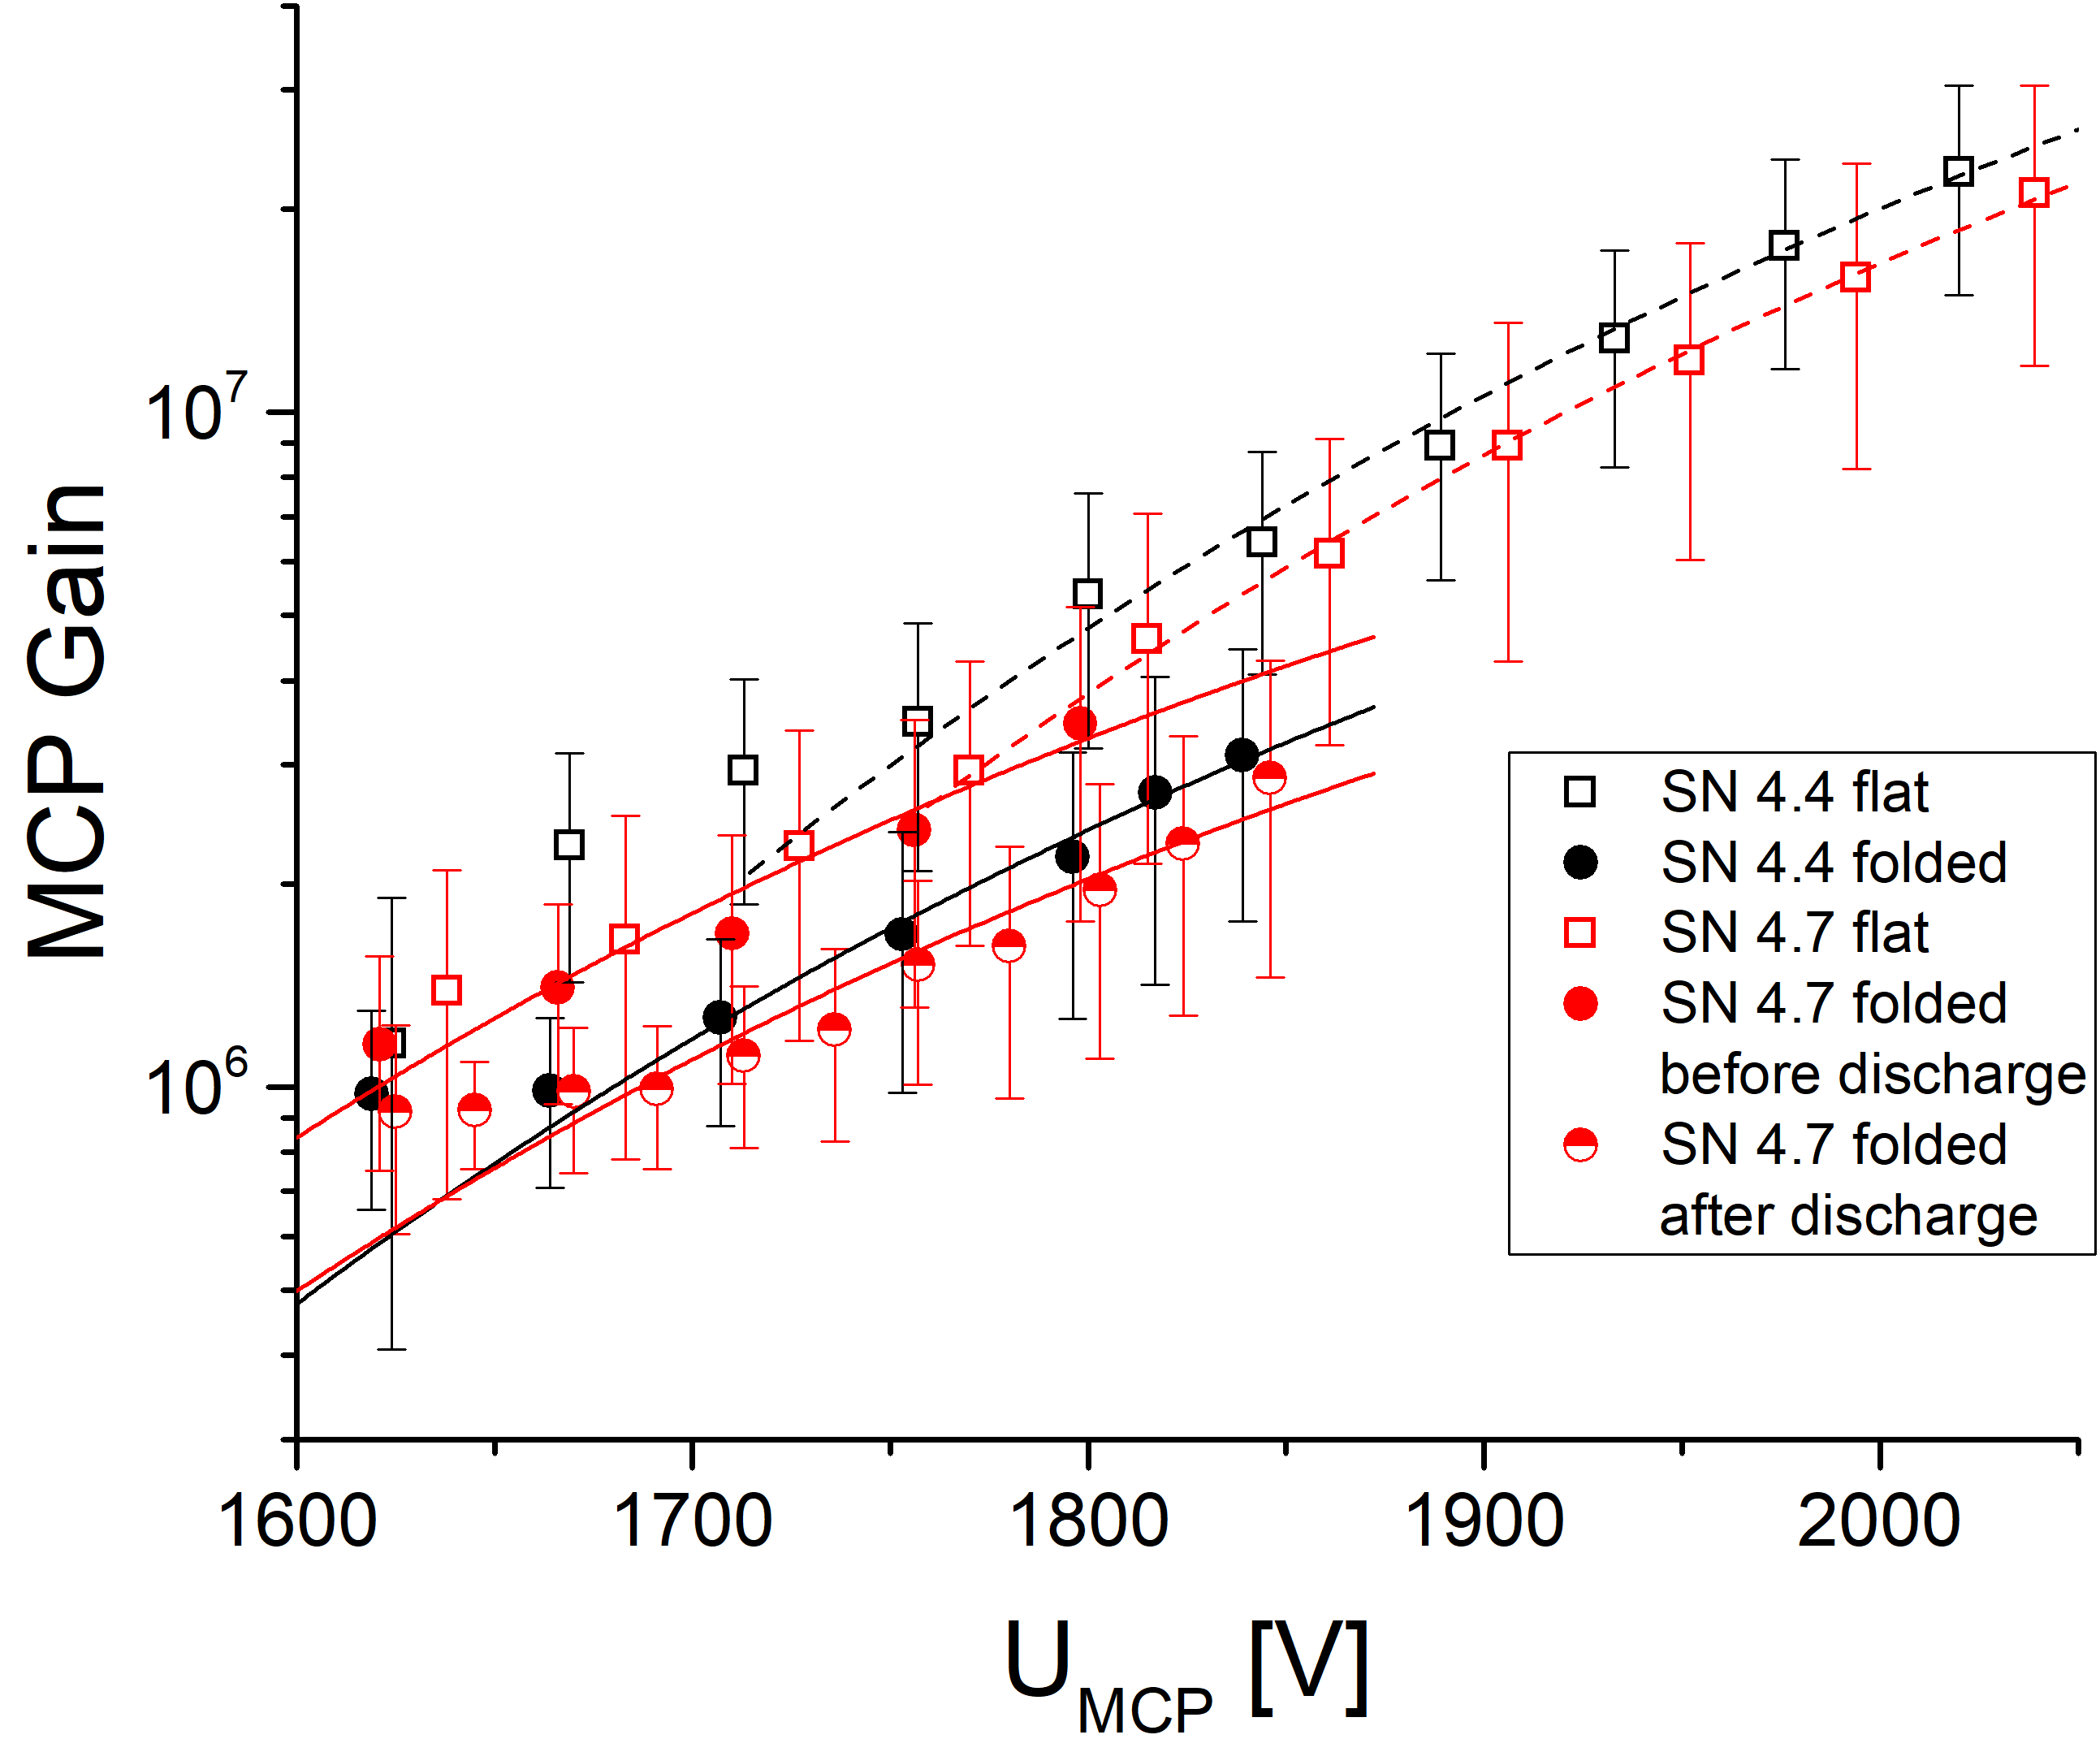
\includegraphics[width=0.9\textwidth]{Experiments/Gain_Curves_SN4p5_4p7.png}
	\end{subfigure}
	\begin{subfigure}{.5\textwidth}
		\centering
		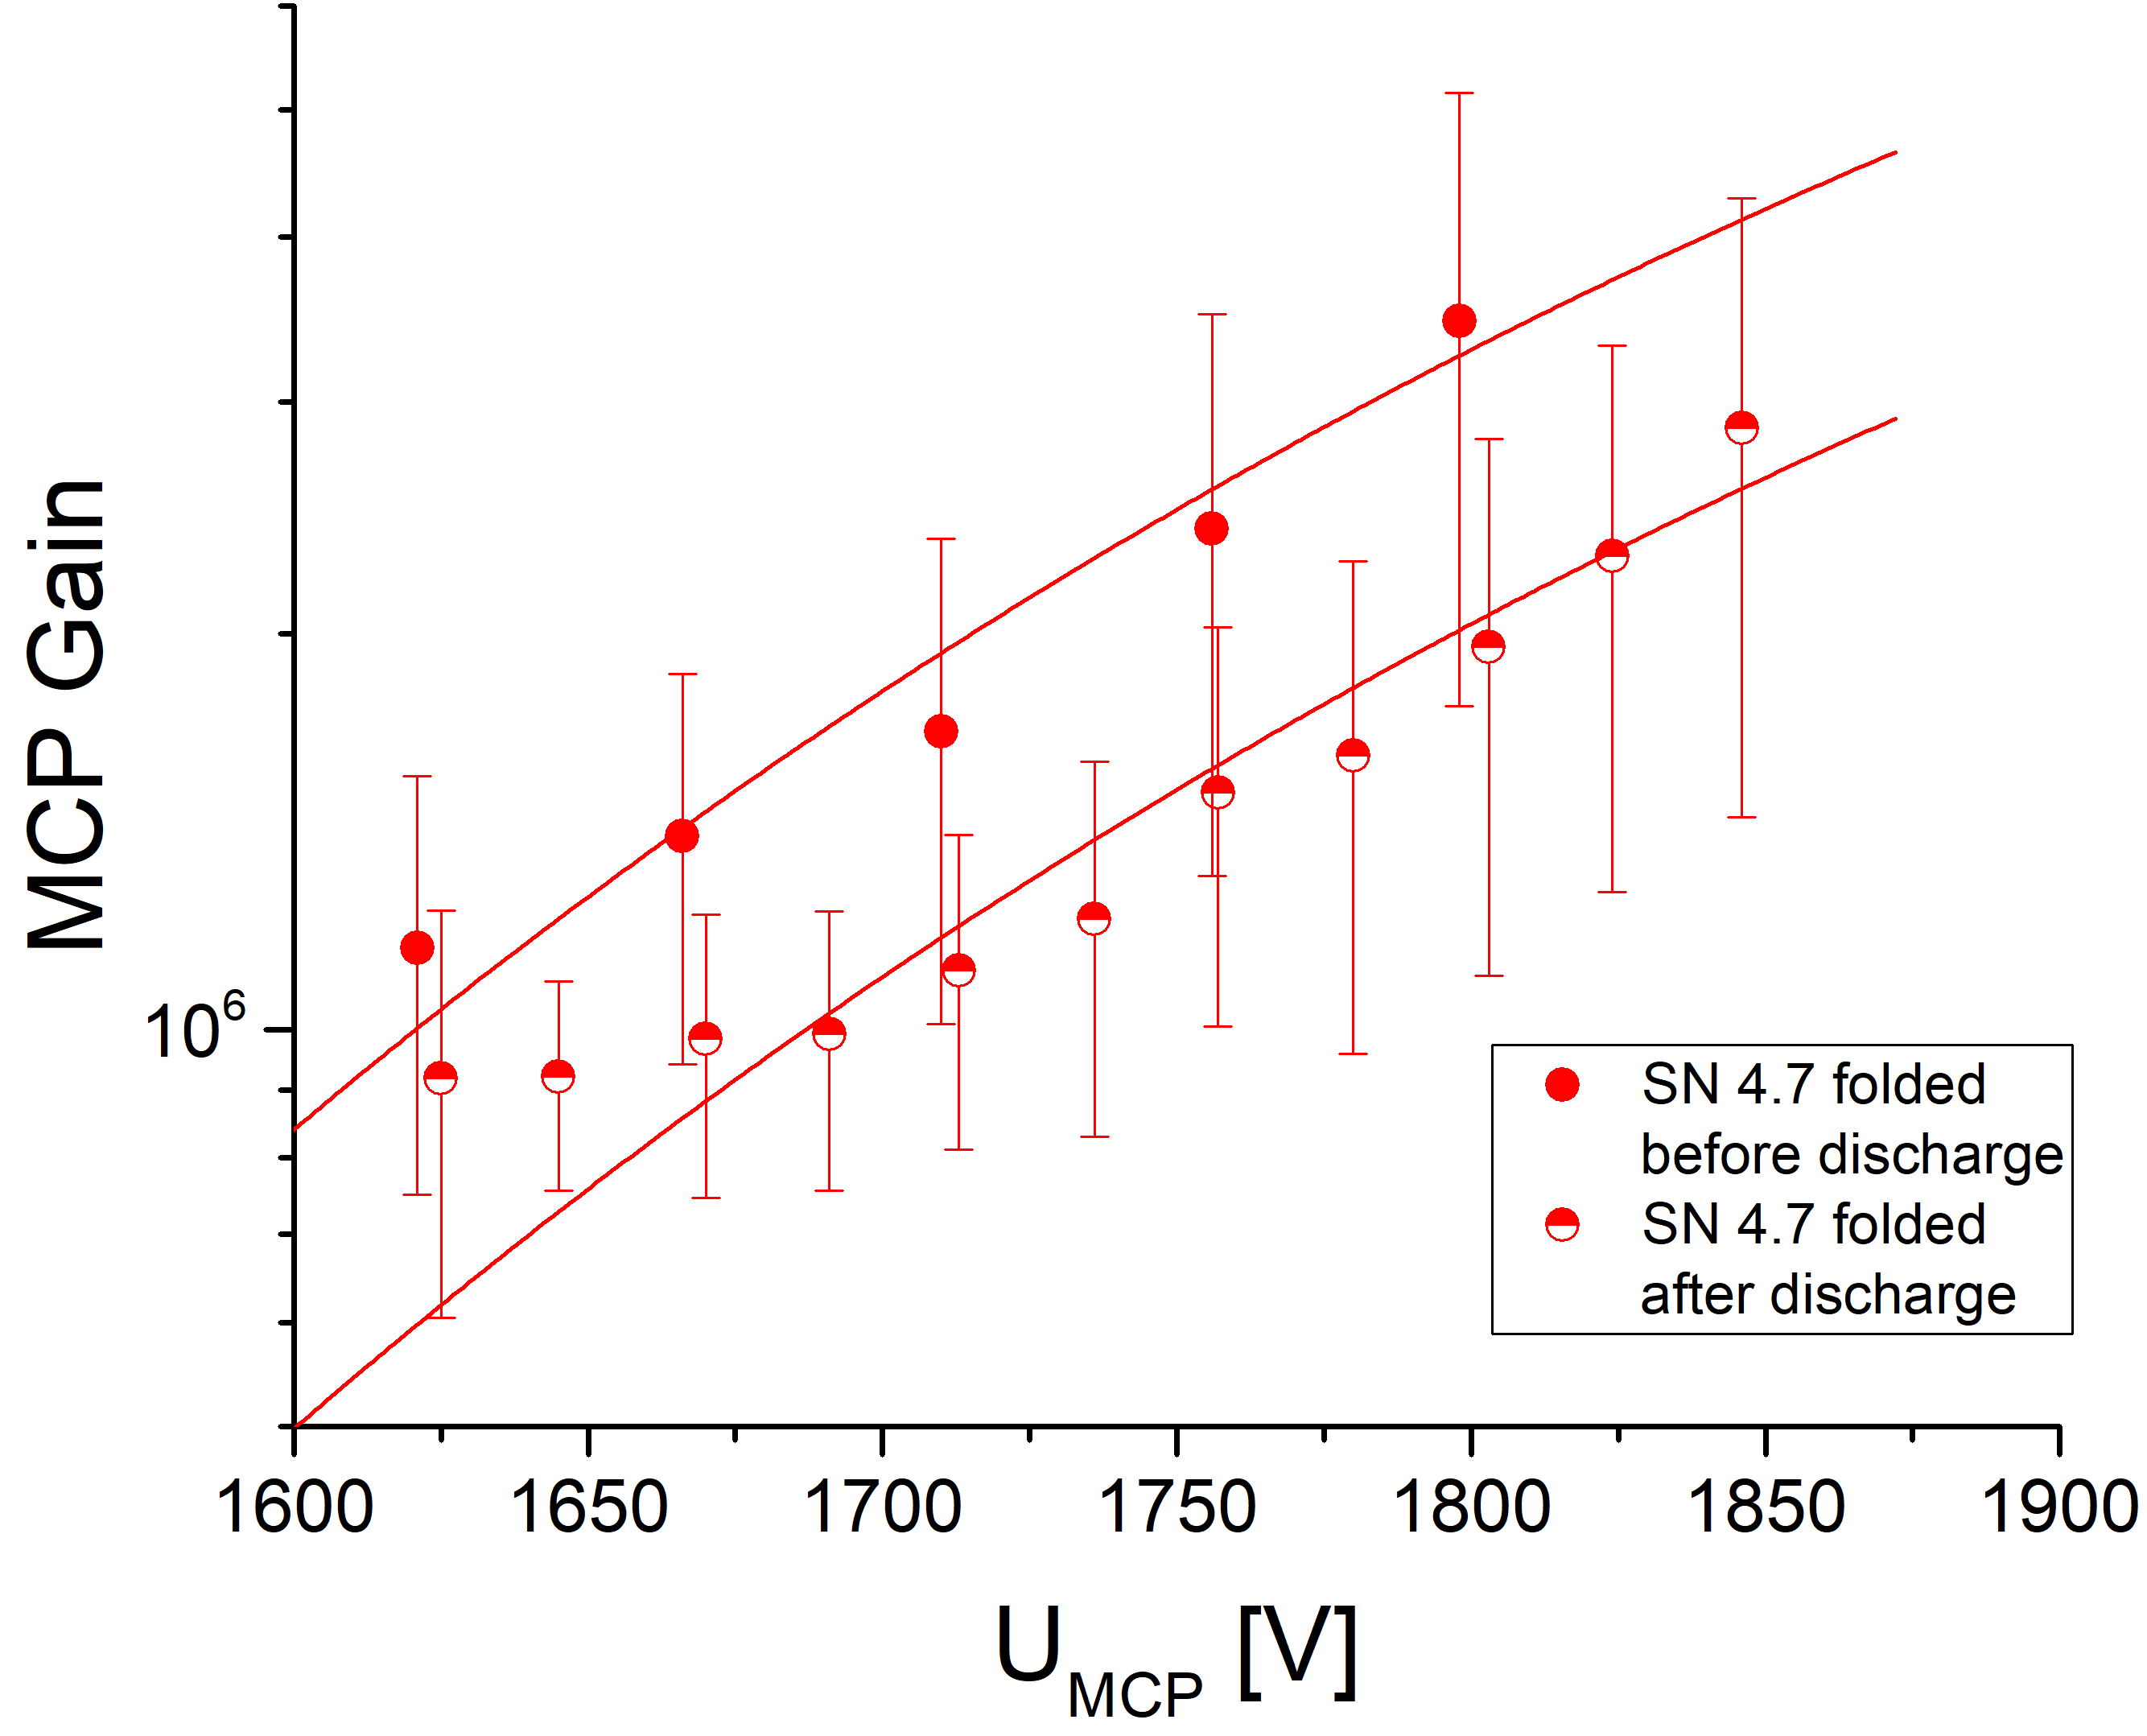
\includegraphics[width=0.9\textwidth]{Experiments/SN4p7_discharge.png}
	\end{subfigure}
		\caption{Left: Gain curves of two NIM PFM detectors. The difference in gain is because for each measurement curve, a different set of MCPs was used. Right: Gain curves of a folded NIM PFM detector. The lower gain curve was recorded after a discharge at an MCP voltage of 1.8\si{\kilo\volt}.}
		\label{fig:SN4p54p7Gain}
	\end{figure}
	\begin{figure}[h] % Theoretical gain curve as a function of time
		\centering
		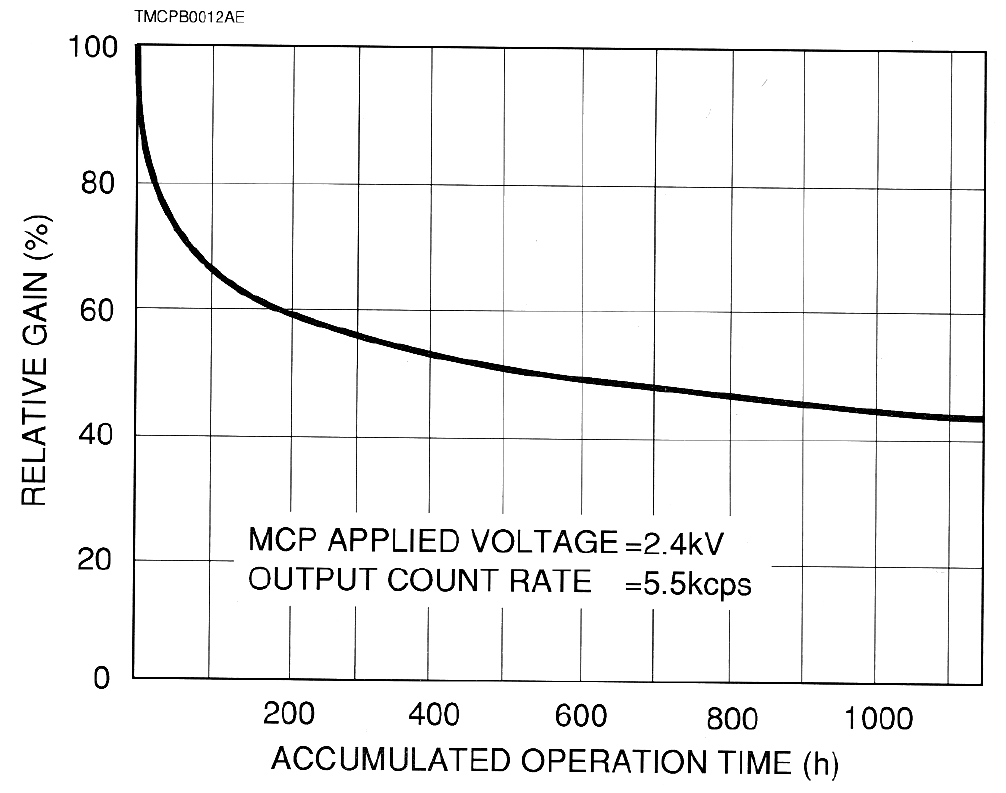
\includegraphics[width=.7\textwidth]{Experiments/MCP_relGain_timeevol.png}
		\caption{Relative gain of an MCP as a function of operation time \cite{LecNot_Wurz2017}.}
		\label{fig:MCPrelGainTime}.
	\end{figure}
	\begin{figure}[h] % FS gain Curve
		\centering
		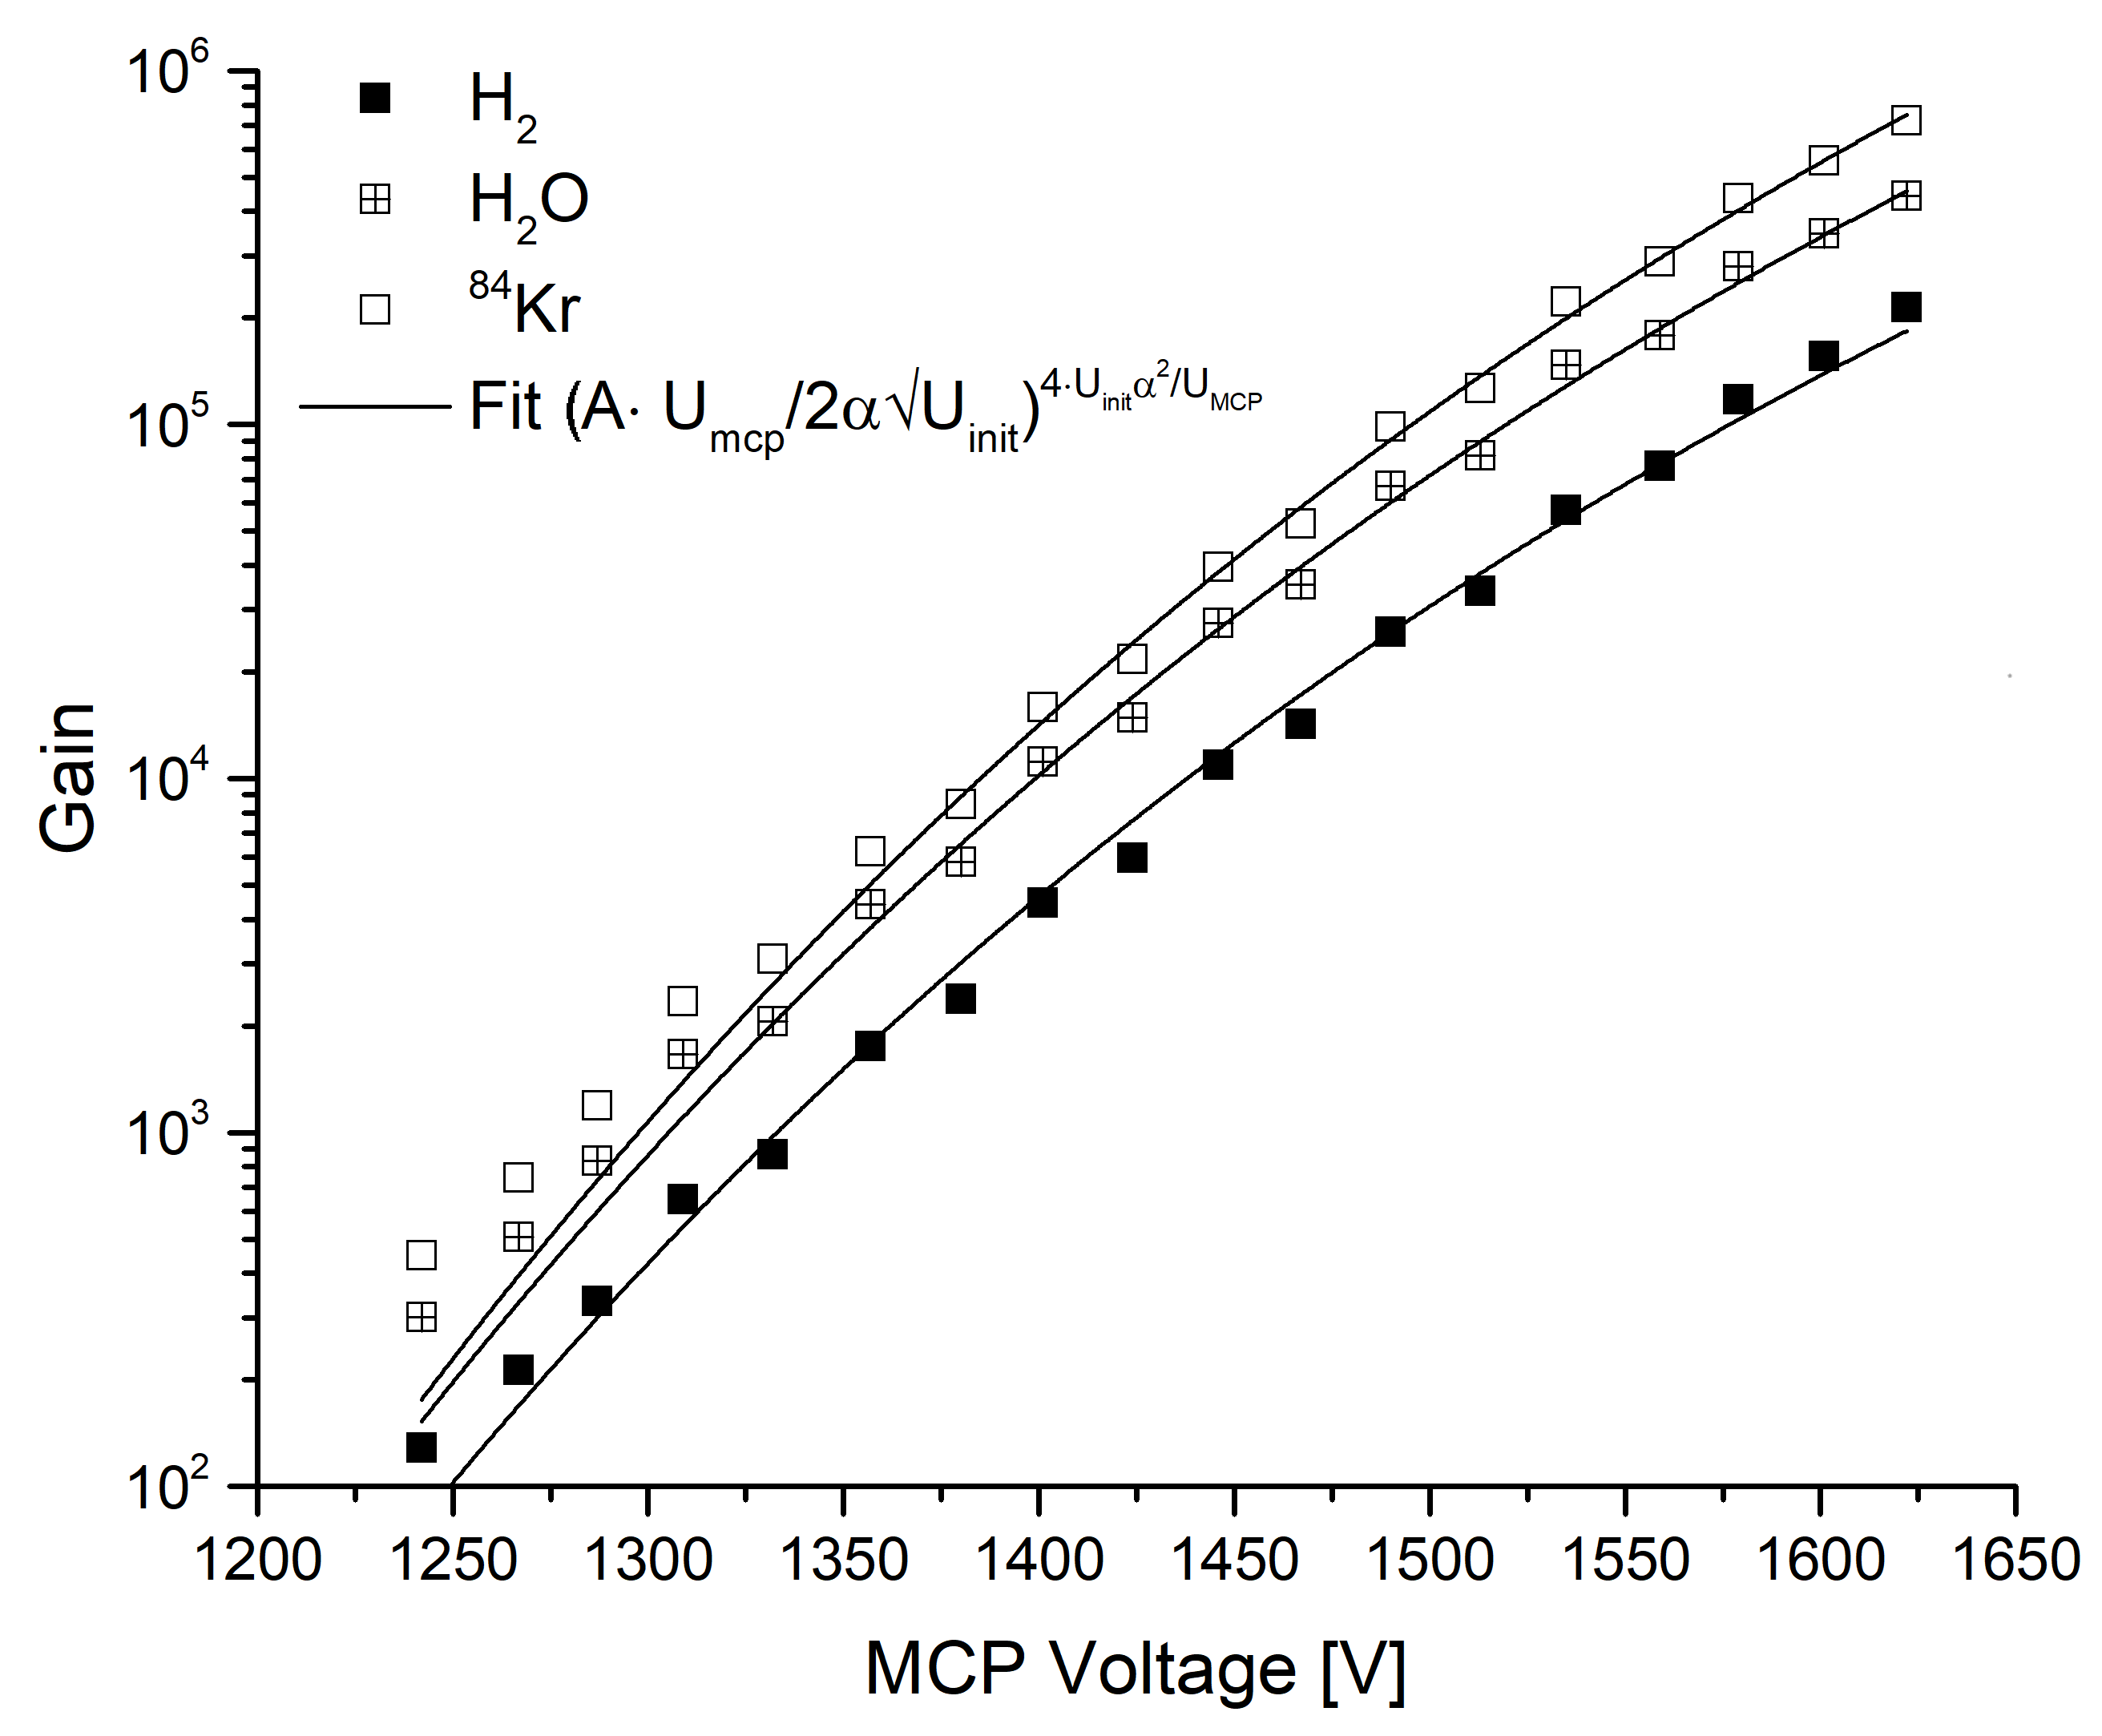
\includegraphics[width=.7\textwidth]{Experiments/GainDetFSLabEl.png}
		\caption{Gain curves measured with the FS instrument.}
		\label{fig:MCPGainCurve4p7}
	\end{figure}
	\begin{figure}[h] % Calibraton curve
		\centering
		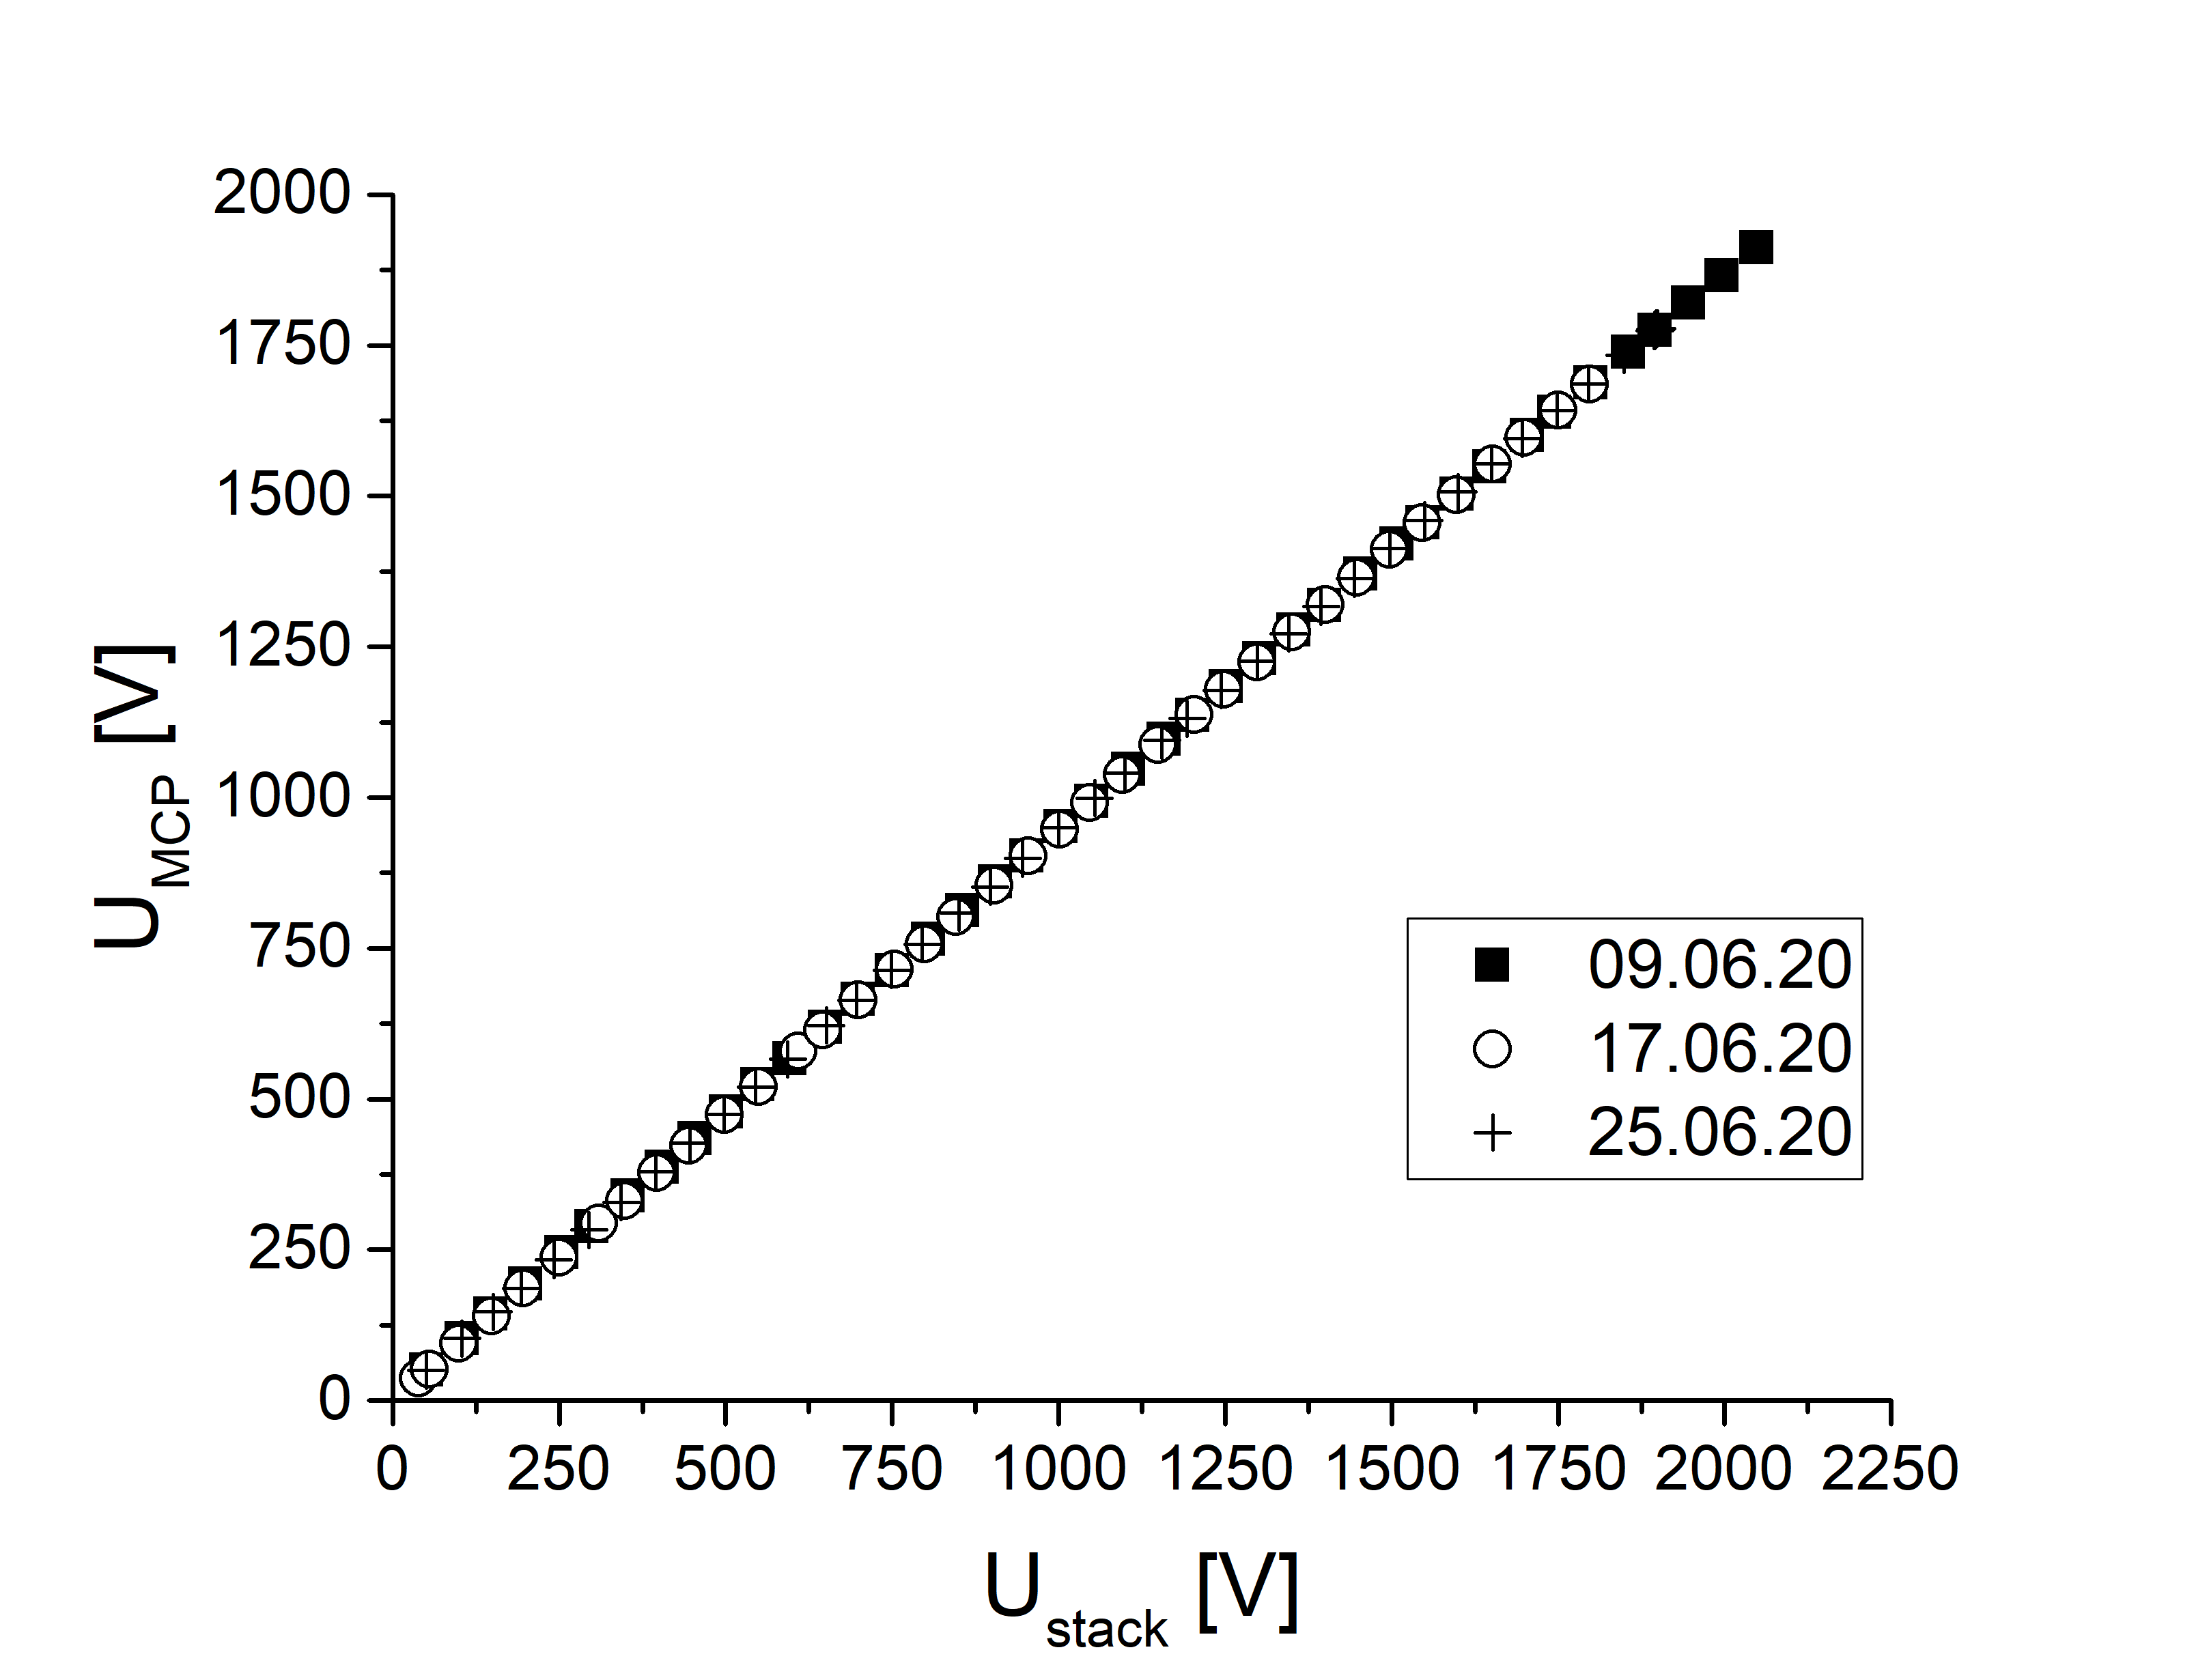
\includegraphics[width=.7\textwidth]{Experiments/PFM_UstackUmccp_TimeEvol.png}
		\caption{MCP voltage (U\textsubscript{MCP}) as a function of the voltage applied between the MCP front and the anode (U\textsubscript{stack}). The fit coefficients of the function $U_{MCP} = a\cdot U_{stack} +b$ are: a = 0.932, b = 12 V.}
		\label{fig:PFMUstackUmcpTimeEvol}
	\end{figure}
	This chapter describes the testing procedure of the flight detectors and shows performance results.\\
	The flight detectors consists of a flexible PCB (Printed Circuit Board) with a peek housing for the MCPs. The flex PCB was needed to reduced the detector volume and therefore to reduced the volume, which has to be shielded against the strong radiation in Jupiter's radiation field. The detectors are tested in flat configuration with test MCPs and in folded configuration with flight MCPs (Fig.\,\ref{fig:DetFlatFolded}). The detectors were put in a vacuum chamber and baked out for 2~days. Earliest one day after bake out, the conditioning was started. The conditioning procedure is attached in the Appendix (Chap.~\ref{sec:appendix}). Depending on the outgas behaviour of the detector, the conditioning took 2.5 to 4.5~h. After the conditioning, the measurements of the detector gain were performed. Fig.\ref{fig:SN4p54p7Gain}~left shows the gain curves of two FS detectors in the two configurations. The conditioning and the measurements in the folded configuration were done up to lower voltages to spare the potential flight MCPs. The gain of the MCPs depends on different factors. As described in chapter~\ref{sec:DetParam} the gain is a function of the voltage applied over the MCPs as it is shown in Fig.~\ref{fig:SN4p54p7Gain}. The MCPs also degrade over time. This process depends on the residual gas pressure at which the MCPs are operated and the residual gas composition. The rapid decline in gain during the first few operation hours is a result of cleaning the channels through operation (Fig.~\ref{fig:MCPrelGainTime}). When the MCPs were exposed to air, water and other substances deposit in the MCP channels. During operation, these deposits are sputtered and the surface of the channels are cleaned. After a few hours, the gain reaches a plateau. % May search here more literature to reference it.
	In flat configuration SN~4.7 has a lower gain than SN~4.4 because its conditioning took longer than the conditioning of detector SN~4.4. Therefore it was cleaned better. In the folded state, SN~4.4 was 3~days longer in vacuum than SN~4.7 and had therefore more time to outgase. Fig.~\ref{fig:SN4p54p7Gain} right shows a zoom on the two measurement series of SN~4.7 both recorded in folded configuration. During the first measurement series, a discharge happened when the MCP voltage was at 1.8~kV. To amplify a signal, a minimal voltage has to be applied over the MCPs. When they are barely used, this voltage is in the range of 1.6~kV. During ageing, the decrease in gain can partially be compensated by increasing the voltage. When an ion induces an electron avalanche, the electrons are free in the channel and their main moving direction is towards the channel output. When a discharge suddenly lowers the applied acceleration voltage, these free electrons get pushed towards the channels walls due to space charge. These electrons destroy the conductive coating leading to a signal reduction of about 30\% per discharge. The higher the applied MCP voltage is, the higher is the signal loss.\\ % Literature. 30% or in that measurement even more depending on which level the discharge happened.
	Fig.~\ref{fig:MCPGainCurve4p7} shows the gain curve of detector SN~4.7 recorded when it was build into the NIM FS instrument. H\textsubscript{2} and H\textsubscript{2}O are part of the residual gas and \textsuperscript{84}Kr is the used test gas. The curves follow nice the theoretical curve. The initial energy of the first electron $U_{init}$ is about 6~eV and the probability $A$ to emit the first electron is in the range of 0.3~eV\textsuperscript{-1/2} for the three species.\\
	Fig.~\ref{fig:PFMUstackUmcpTimeEvol} shows the relation between the voltage applied over the MCPs $U_{MCP}$ as a function of the voltage $U_{stack}$ applied between the MCP front and the anode for the PFM and the FS detector. The MCPs in the two detectors have similar resistances. Therefore, the FS detector can be used to analyse the long term behaviour. Due to the similar resistances, the measurement data of the two detectors overlap. For the PFM detector, a longer measurement campaign was done to characterize the PFM instrument (Chap.~\ref{sec:paper}). During that campaign, this curve was recorded frequently every time the instrument was turned on. The resistance did not seem to change during the short time of the measurement campaign.
	
	% Measuring settings. Turn the drift voltage up to -2.5 kV and then slowly increase the anode voltage to the value you want to measure. The gain is calculated with the software by doing a Simpson 3/8 integration of the peak = Q.

	% Discharge pulse shape discussion.
	% Detector with broken anode is detector EM4. Look if there are any specifications. Seems to have most probable the same configuration as the other detectors. -> Sufficient for the data analysis but it would be good to have the datasheet.	
	% Fig. \notes{bla} shows the signal shapes of different detector configurations beginning with the shape of a detector with a broken diode. The other figure shows the signal shape of a detector with a functioning resistor. The most remarkable feature is that the signal height of the detector is much smaller and much broader that the signal shape of the other configurations. In addition, the first overshoot is much lager due to the impedance mismatch caused by the broken diode. A broken diode gets conductive and therefore the potential at the MCP backside is equal to the potential of the anode. The electrons are not additionally accelerated and therefore the resulting signal is smaller than the signal with a functioning diode.\\

		
%---------------------------------------------------------------------------------------------	
	\subsection{Sensor performance tests}
		This chapter shows the performance of the NIM PFM and the NIM FS sensor when operated with laboratory electronics.
		
		\subsubsection{PFM}\label{sec:paper}
		\notes{Include IEEE paper!!!}.
		\subsubsection{FS \notes{finished}}
	
		\textbf{Ion Storage}\\ % Ref. to Abplanalp paper.
		Ion storage is very crucial for a time of flight mass spectrometer because every ion generated and not stored in the ion source is lost and can generate additional electrical noise on the detector signal line. In this test the ion storage behaviour of the ion source was analysed for thermal and neutral mode for hydrogen and krypton with velocities of 2\,\si{\kilo\meter\per\second} and 4\,\si{\kilo\meter\per\second}. The emission current was varied from 20 to 600\,\si{\micro\ampere}. Ion storage of positive ions in x- and y- direction is supported by the negative potential generated by the electron beam. Two ring electrodes with a positive voltage applied generate a positive potential ring to trap generated ions in y- and z- direction (Fig.\ref{fig:ExpFSFlightSenIonStorIS}). For emission currents from 20 to 600\,\si{\micro\ampere} according to Eq.\,\eqref{eq:elPotIem} the negative potential in the centre of the electron beam is -0.08-(-2.59)\,\si{\volt}. Fig.\ref{fig:ExpFSFlightSenIonStor} left shows the ion storage behaviour of the ion source of hydrogen and right the ion storage behaviour of krypton. In case of no ion storage, the relationship between the electron emission current I\textsubscript{em} and the signal intensity is linear. In case of ion storage there is a quadratic relationship between I\textsubscript{em} and the signal intensity. When measuring with the thermal mode, the particles get slowed down until they have energies in the range of 0.01\,\si{\electronvolt} and are therefore easy to trap in the potential field. When measuring with the neutral mode, particles enter the ionisation region directly. The kinetic energy of hydrogen for velocities between 2-4\,km/s is 0.07-0.27\,eV. Therefore it can be trapped with the potential field generated by an electron beam with an emission current higher than 20~$\mu$A.\\
		The kinetic energy of \textsuperscript{84}Kr for the same velocities is 2.8-11.2\,eV. This energy exceeds the potential of the centre of the electron beam and the ions are therefore more difficult to trap with only the electron beam. The ions are kept in the middle of the ionisation region with the positive potential ring. According to Fig.\,\ref{fig:ExpFSFlightSenIonStor} ion storage for \textsuperscript{84}Kr starts to dominate at emission currents higher than 100\,$\mu$A. In thermal mode, an increase in beam velocity leads to an increase in signal intensity due to the density enhancement effect (Chap.\,\ref{subsubsec:Densenhan}). Therefore a higher signal intensity is expected in thermal mode for 4\,km/s compared to 2\,km/s. Like in the PFM, the FS shows a nice ion storage behaviour. For krypton ion storage just starts at an emission current of 100\,\si{\micro\ampere} where hydrogen is stored already at lower emission currents due its lower kinetic energy at the same beam velocity.\\
		\begin{figure}[h]
			\centering
			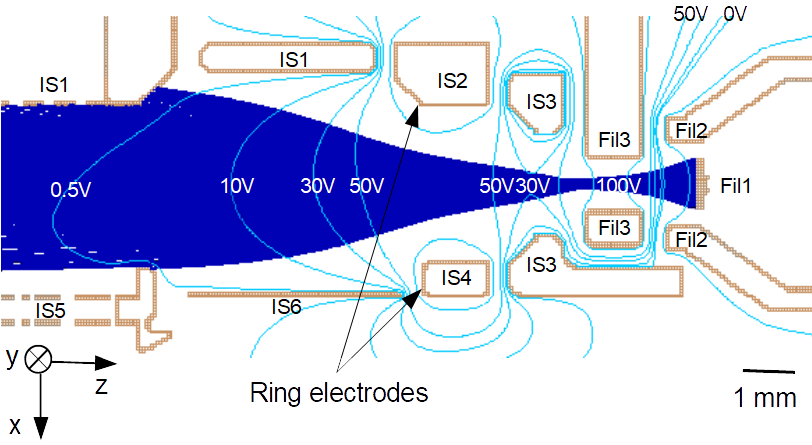
\includegraphics[width = 0.7\textwidth]{Experiments/FiL_IS_elBeam_Storage.png}
			\caption{Ion storage source with sample voltage set applied to the electrodes. In light blue are the potential lines and in dark blue a simulated electron beam.}
			\label{fig:ExpFSFlightSenIonStorIS}
		\end{figure}
		\begin{figure}[h] % Split in 2 Picutres? Because it is very small
			\begin{subfigure}{0.5\textwidth}
				\centering
				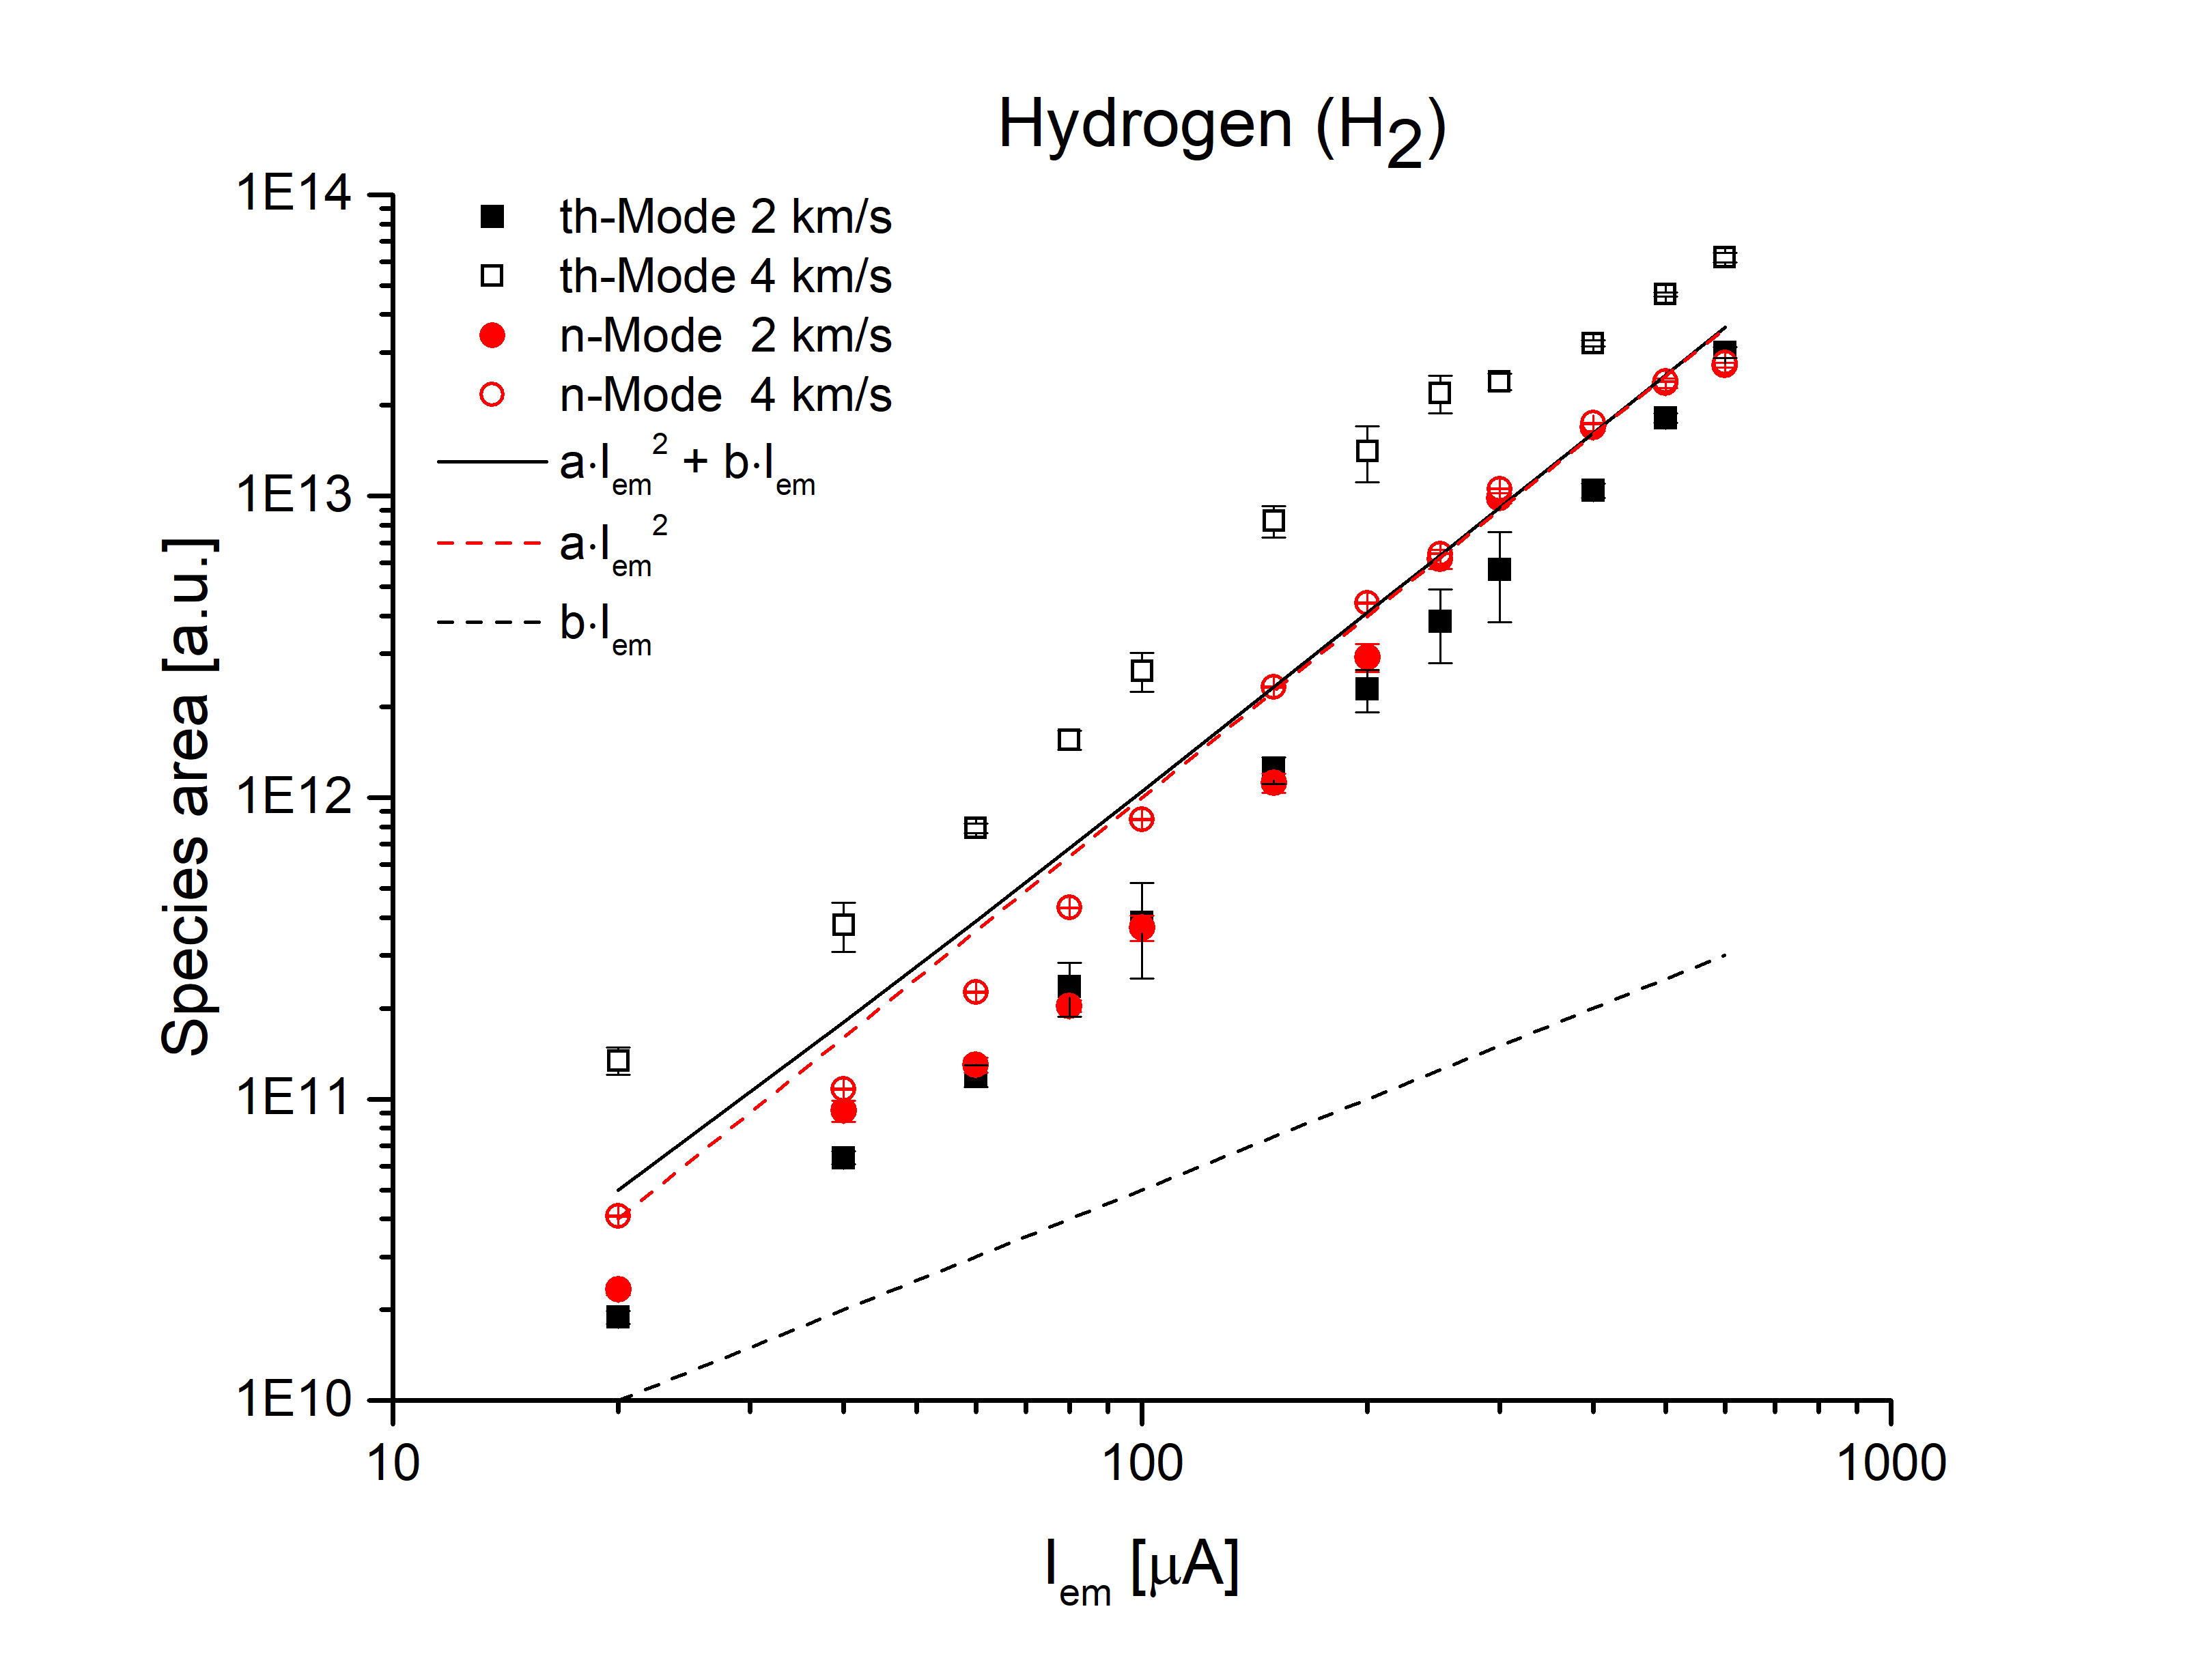
\includegraphics[width = \textwidth]{Experiments/FSLabIonStorageH2.png}
			\end{subfigure}
			\begin{subfigure}{0.5\textwidth}
				\centering
				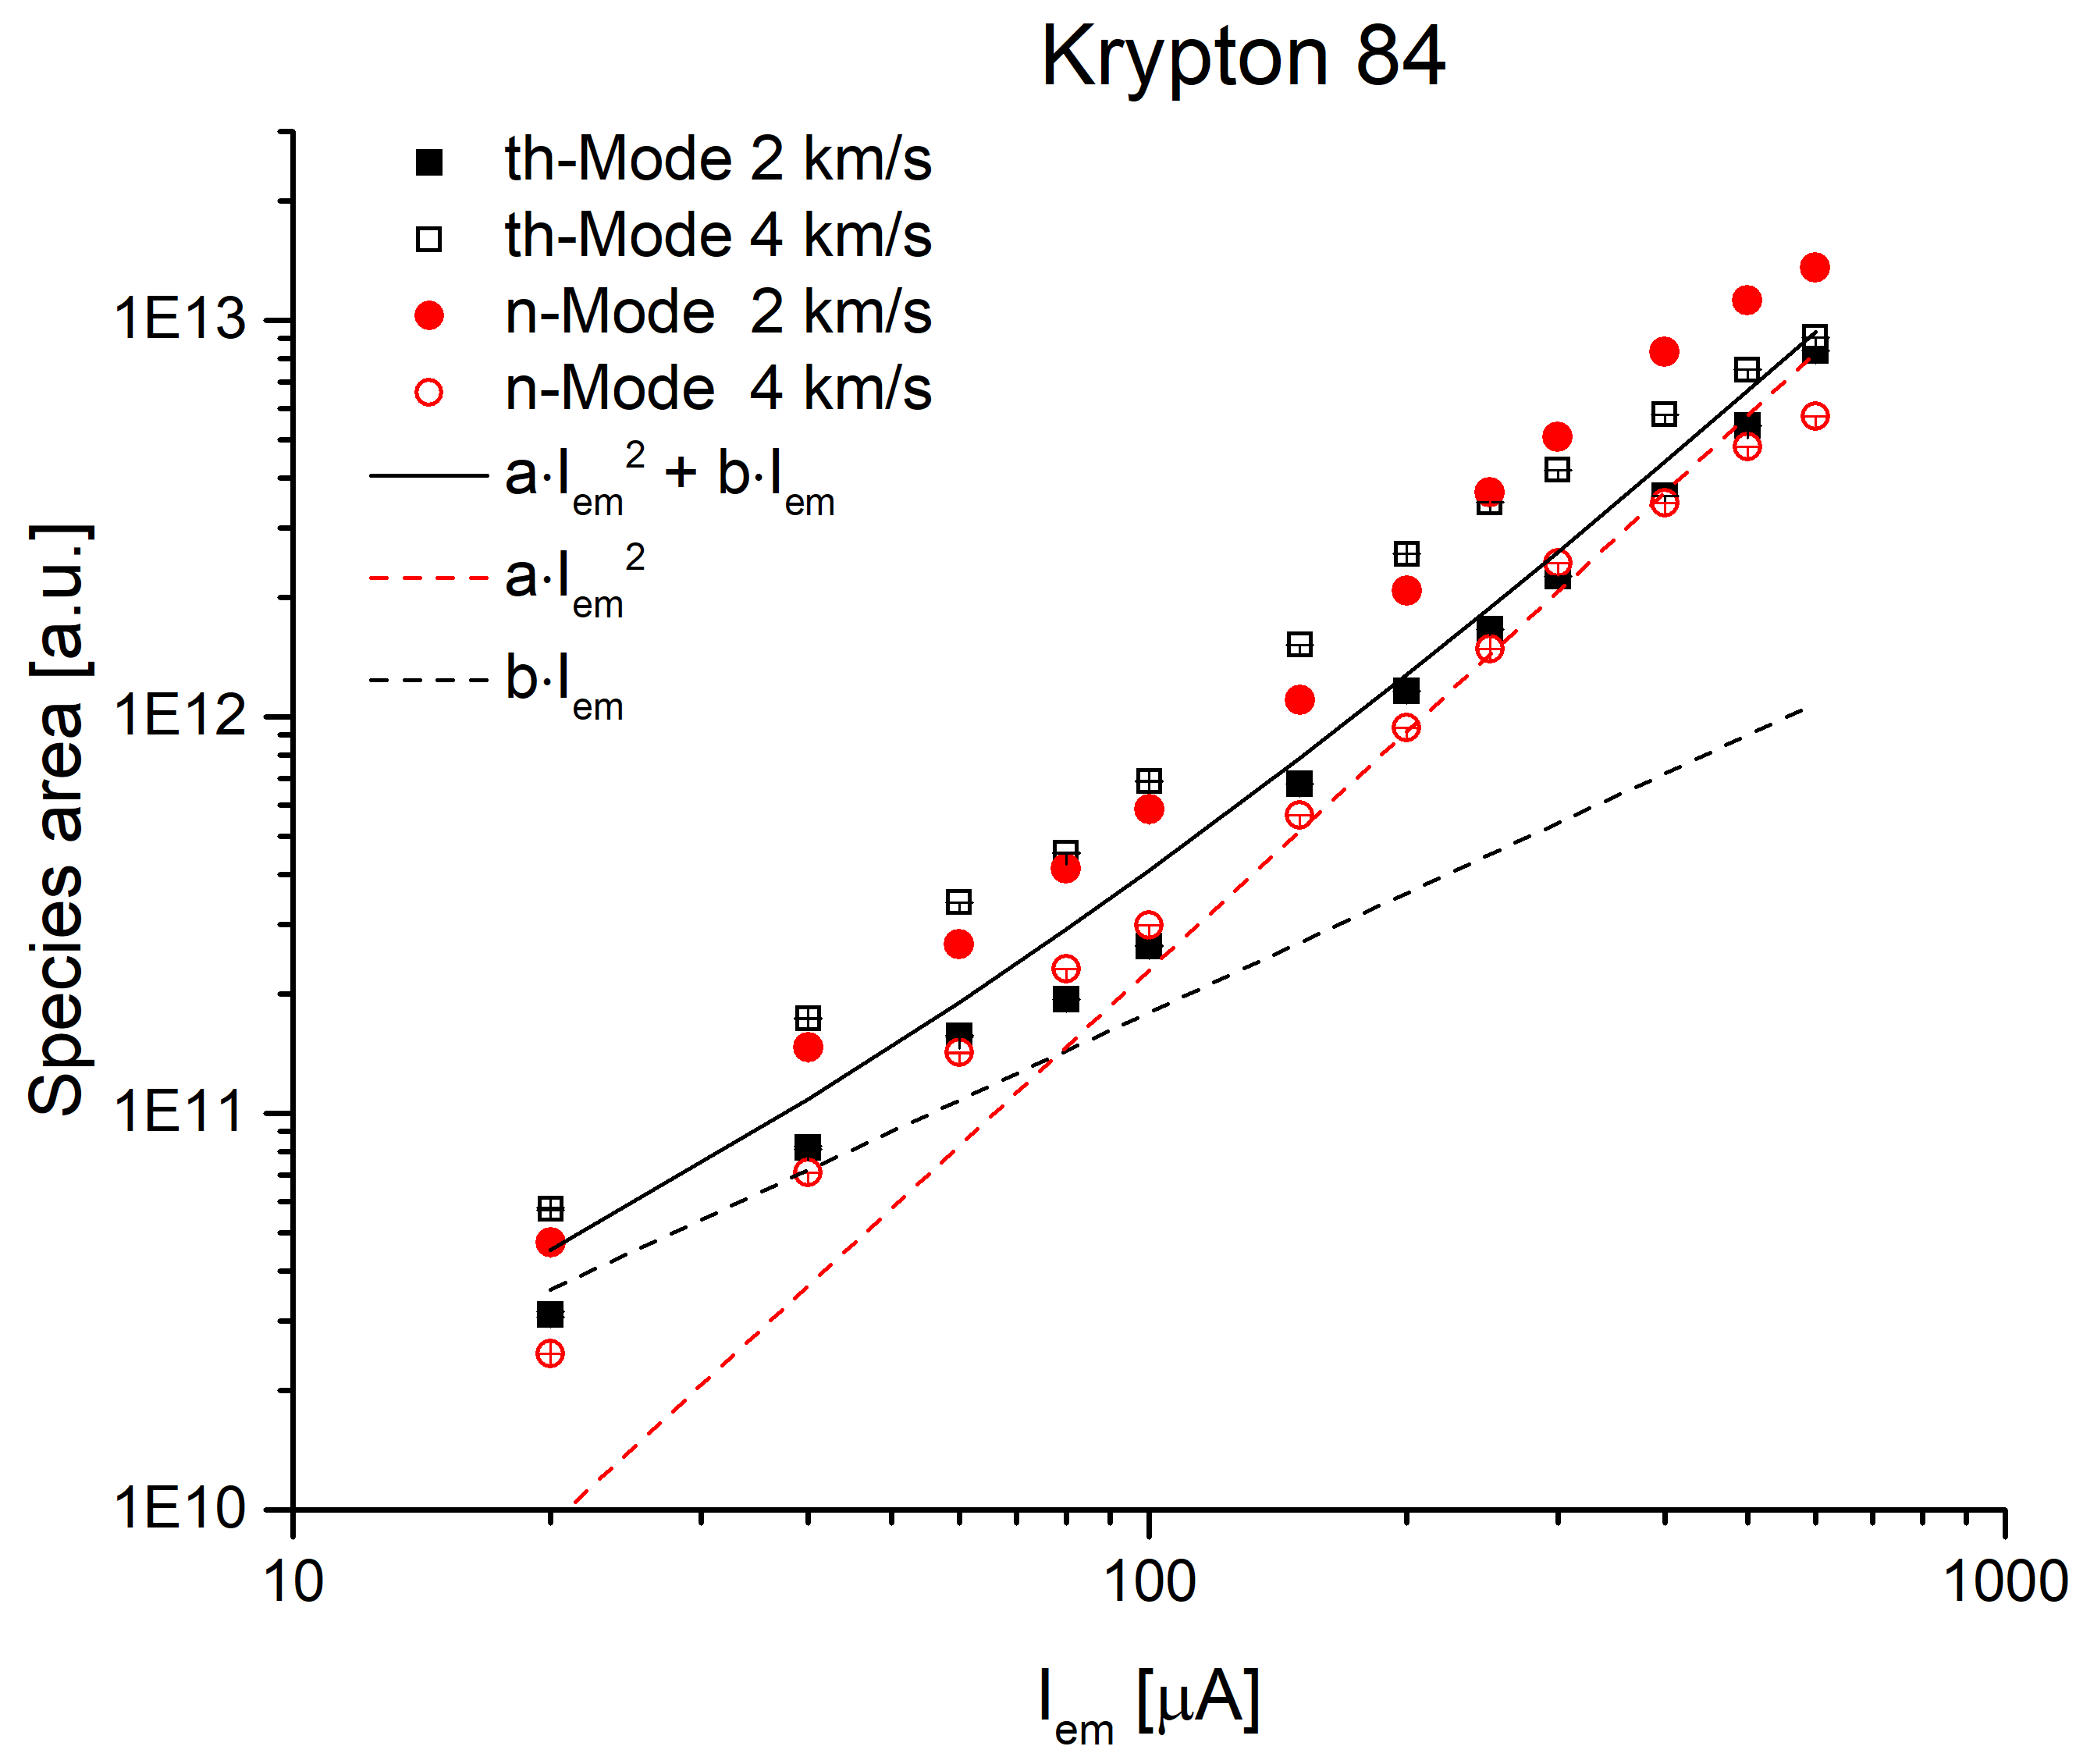
\includegraphics[width = \textwidth]{Experiments/FSLabIonStorageKr84.png}
			\end{subfigure}
			\caption{Ion storage measurements performed with the flight spare sensor operated with laboratory electronics for H$_2$ and $^{84}$Kr for two different gas velocities.}
			\label{fig:ExpFSFlightSenIonStor}
		\end{figure}
		
		\textbf{Mass resolution and Signal-to-Noise Ratio}\\
		According to the requirements stated in \cite{red_book} NIM has to achieve a mass resolution for neutral mode of 500 and for thermal mode of 1000 but to be able to distinguish between different masses at unit masses of 1000\,m/z NIM has to have a mass resolution of 1000. Otherwise, the different unit masses cannot be distinguished.\\
		Fig.\,\ref{fig:ExpFSFlightSenMassRes} shows two spectra recorded with the NIM~FS sensor with laboratory electronics attached with an electron emission current of 100\,$\mu$A. With a mass resolution of 708 for neutral gas mode NIM fulfils the requirements. In thermal gas mode the highest mass resolution achieved was 830 m/$\Delta$m. Fig.\,\ref{fig:ExpFSFlightElMassRes} shows mass spectra recorded with the NIM~FS sensor with the flight electronics attached. The electron emission current was 200\,$\mu$A. The highest mass resolution achieved at the current state is 490 m/$\Delta$m for neutral gas mode and 462 m/$\Delta$m for thermal mode. The mass resolution can be improved by further optimizing the system. With an emission current of 300\,$\mu$ the \textsuperscript{78}Kr isotope is visible in the spectrum which has a natural abundance of 0.36\,\% (Fig.\,\ref{fig:ExpFSFlightElK78}).\\
		The signal to noise ratio for the spectra recorded with the flight electronics is very low compared to the SNR of the spectra recorded with the laboratory electronics. The SNR can be improved by adding proper noise filters.	A wandering noisy part is already identified. In Fig.\,\ref{fig:ExpFSFlightElMassRes} left and right it appears between masses m/z 40 and 70. In Fig.\,\ref{fig:ExpFSFlightElK78} it start right after the noise of the extraction pulse an ends at m/z 30. At the moment it is unclear what induces that noise but with a proper filter this noise can be detected and significantly reduced without affecting the mass signal peaks.\\
		Fig.\,\ref{fig:ExpFSFlightSenSNR} shows a mass spectrum recorded with the FS sensor with the laboratory electronics attached. The highest SNR achieved was $6\cdot10^{5}$ and therefore almost 6 decades. The mass peaks m/z 355, 390 and 429 are some oil components with water adducts originating from the turbo pumps of the test facility. m/z 415 is an artefact generated by the algorithm used for the background subtraction. This peak is also wider then the other surrounding mass peaks.
		A SNR of 6 decades is important to conduct optimal measurements during the flybys at Jupiter's icy moon Europa. The particle density of Europa's exosphere is about 10~-~10\textsuperscript{8}~cm\textsuperscript{-3} \cite{Vorburger_2018} corresponding to a pressure of 10\textsuperscript{-15}~-~10\textsuperscript{-8}~mbar. With a chamber pressure of 1.5$\cdot$10\textsuperscript{-9}~mbar NIM has to achieve a SNR of 6 decades to measure particles at a pressure of 10\textsuperscript{-15}~mbar.
		\begin{figure}[h]
			\begin{subfigure}{0.5\textwidth}
				\centering
				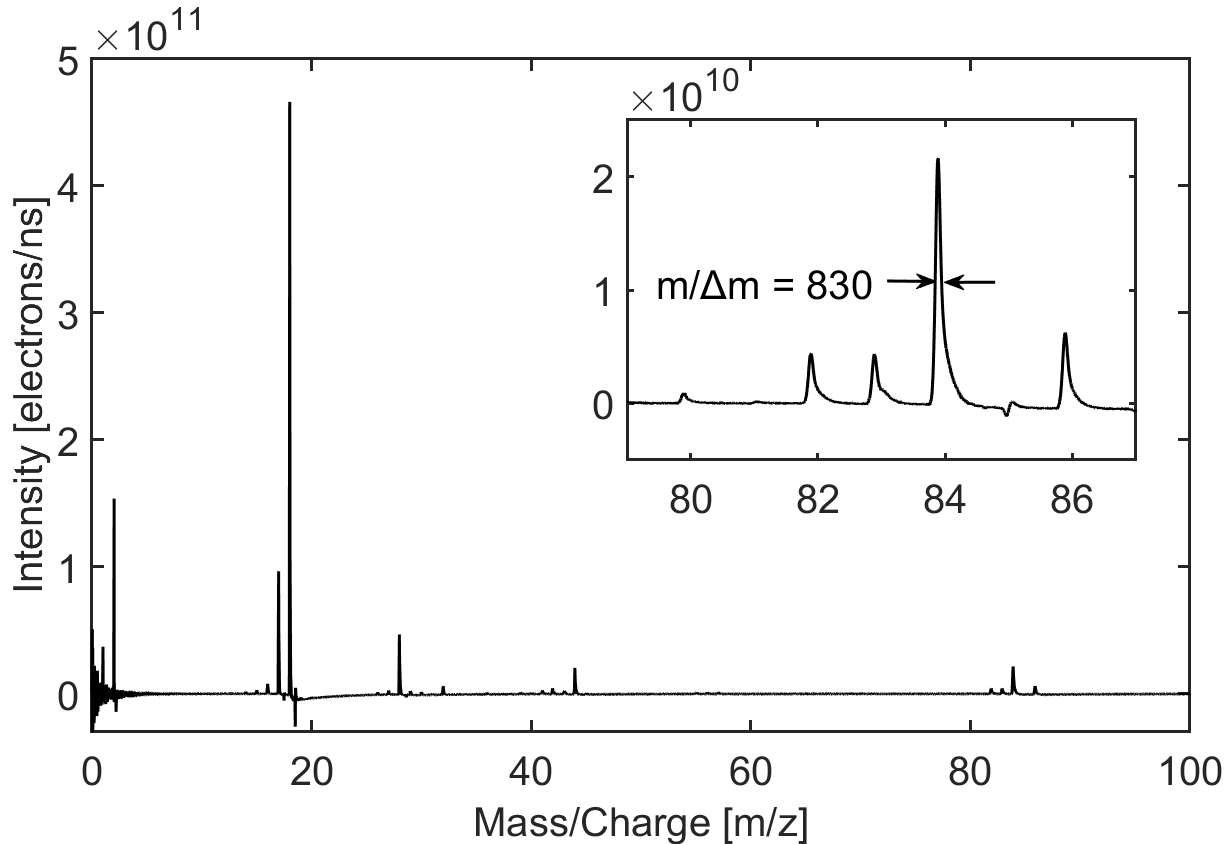
\includegraphics[width = \textwidth]{Experiments/FSLabthMode.png}
			\end{subfigure}
			\begin{subfigure}{0.5\textwidth}
				\centering
				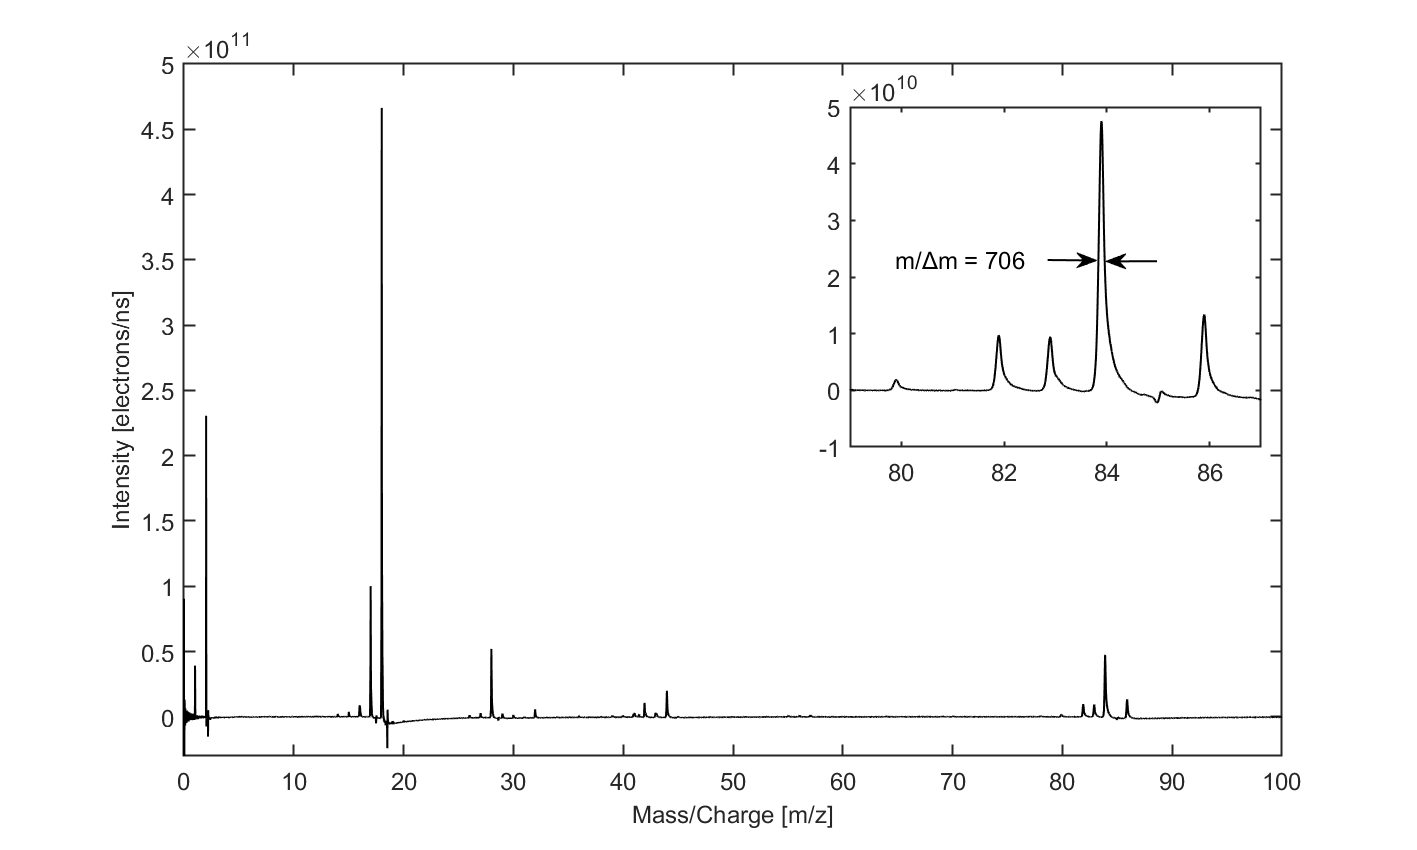
\includegraphics[width = \textwidth]{Experiments/FSLabnMode.png}
			\end{subfigure}
			\caption{Mass spectra measured with the flight spare sensor with the laboratory electronics attached. Left: thermal gas mode. Right: neutral mode.}
			\label{fig:ExpFSFlightSenMassRes}
		\end{figure}

		% Mark the noisy part for better description to explain that
		% conditions: nMode UMCP: 1950 V. P = 1.03e-8 mbar 20H2:1Kr
		%			thMode UMCP = 1950 V. P = 6.05e-8 mbar
		\begin{figure}[h]
			\begin{subfigure}{0.5\textwidth}
				\centering
				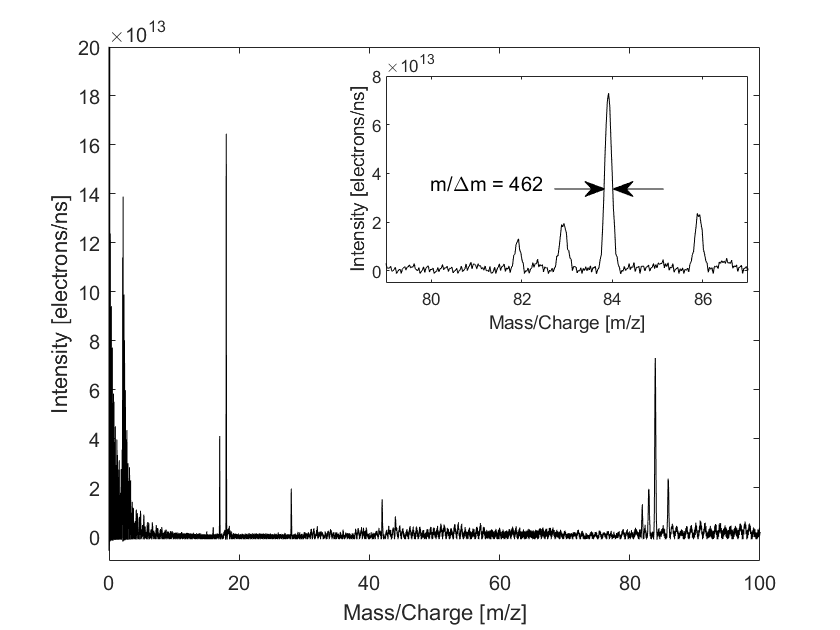
\includegraphics[width = \textwidth]{Experiments/FSthMode200uA.png}
			\end{subfigure}
			\begin{subfigure}{0.5\textwidth}
				\centering
				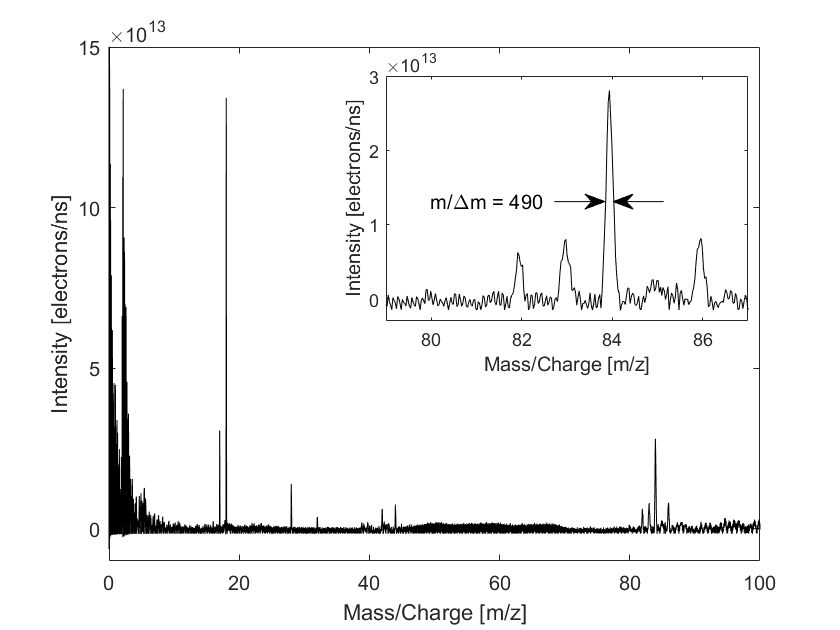
\includegraphics[width = \textwidth]{Experiments/FSnMode200uA.png}
			\end{subfigure}
			\caption{Mass spectra measured with the flight spare instrument with the flight electronics attached. Filament emission current was 200\,$\mu$A. Left: thermal gas mode. Right: neutral mode.}
			\label{fig:ExpFSFlightElMassRes}
		\end{figure}
		
		\begin{figure} % Point out at that picture that the Kr 78 isotope is clearly visible.
			\centering
			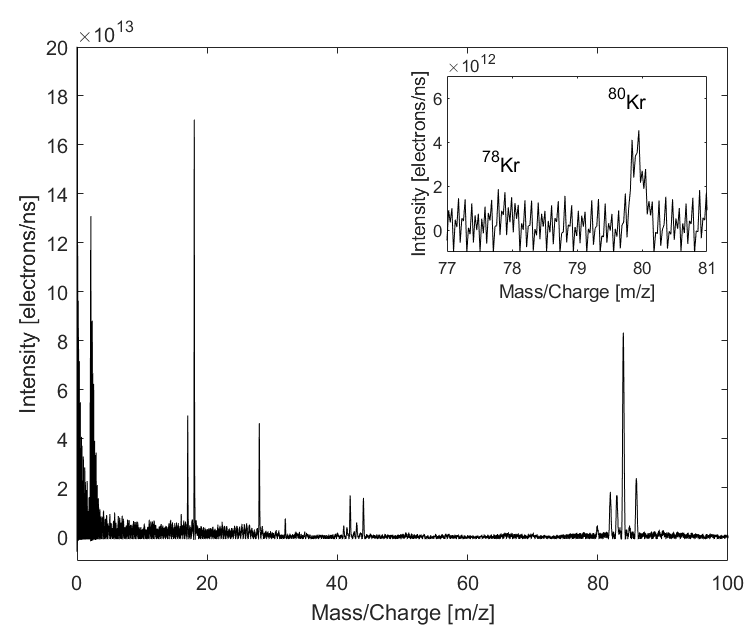
\includegraphics[width = 0.6\textwidth]{Experiments/FS_thMode300uA.png}
			\caption{Mass spectrum measured with the flight spare instrument with the flight electronics attached with a filament emission current of 300\,$\mu$A.}
			\label{fig:ExpFSFlightElK78}
		\end{figure}
		
		% SNR 600 uA emission current. Rest gas Ptot = 1.6e-9 mbar, UMCPeff = 1.8 kV. Name the gas peaks. Peaks around 200 u are not mercury because the isotopic ratio does not match the pattern.
		\begin{figure}[h]
			\centering
			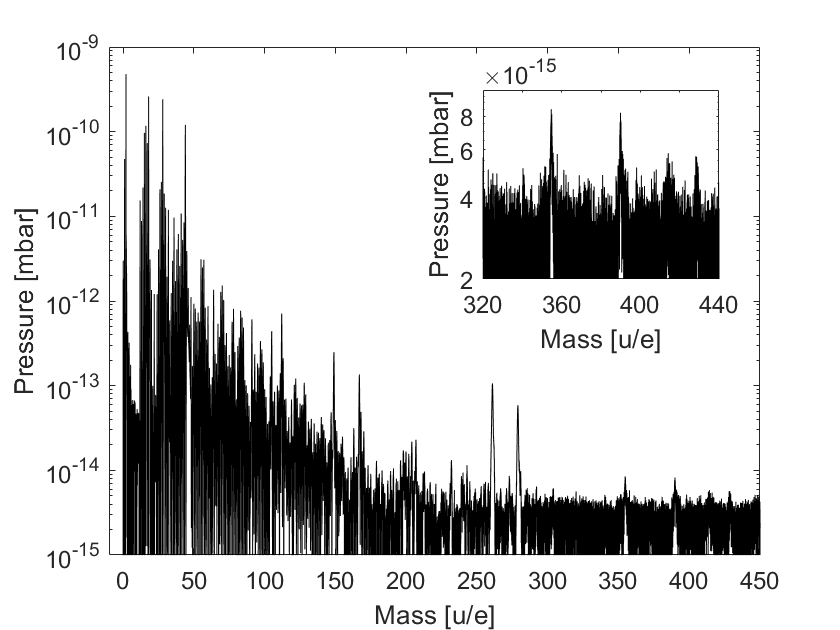
\includegraphics[width = 0.7\textwidth]{Experiments/FSLabSNRRestGasPressCal.png}
			\caption{SNR plot for the flight spare sensor but with laboratory electronics attached. The residual gas pressure was 1.5$\cdot$10\textsuperscript{-9}\,mbar.}
			\label{fig:ExpFSFlightSenSNR}
		\end{figure}
	
	
	
	
	
	
	